\chapter{A Critical Comparison of \AbInitio\ Methods for Loop Modelling}
\label{chapter:methods}

\begin{quote}
``As a scientist, Throckmorton knew that if he were ever to break wind in the echo chamber, he would never hear the end of it.''\\
--- \textit{Bulwer-Lytton Fiction Contest, San Jose University, California}
\end{quote}

\section{Introduction}

Loop regions in protein structures are the ideal test case for any conformational
search method and associated forcefield due to their short length, structural variability, and weak sequence$\to$structure relationships. General lessons learned from sampling
the conformational space of loop structure are likely to be applicable to
protein modelling as a whole.

As has already been discussed in chapter \ref{chapter:database}, the PDB contains sufficient data to well represent shorter loop classes of up to seven residues in length\cite{METHOD:Fid94}.
Existing database methodologies have been shown to be both extremely rapid and very capable at modelling these shorter classes of simple loop; although there is room for improvement. For loops and compound loops greater in length than seven residues, the database methodology begins to fail in terms of data coverage for  both sequence and
conformational space. As such, \abinitio\ methods are the logical choice for longer classes of loop.
The focus of the method development for this thesis has been the modelling of medium-to-long length loops, which are defined here as those between 6 and 12 residues in length. This size of loop is, therefore, the focus of this critical method comparison.

Although individual publications quote prediction success rates, they commonly
use a limited
number of candidate structures and vary in the exact score of success. As
such, when reviewing the literature, it is difficult to quantify the relative
performance characteristics between individual methods.  Ideally one would
compare each method on the same large test-set of loops and rank them via the same
score. Such a comprehensive critical comparison of loop modelling methods has not yet been reported in the literature. 



It was the ultimate goal of this review to accomplish this by systematically comparing several \abinitio\ loop modelling methods on a large representative test-set. Use of the most comprehensive loop database to date, described in section \ref{section:intro:loop_db}, facilitated the collection of statistically significant performance data for each method. The chosen published methods for evaluation are described in section \ref{section:methcomp:methodlist}.  




\subsection{Use of the \uobf}

Throughout this comparison, the \uobf\ has been extensively used, specifically the methodology assembly described previously in section \ref{section:uobf:methodology}. In essence, to manage all matters pertaining to each assessed method, multiple classes were derived from the base-class described in listing \ref{listing:db:dsspcode}, where each used data from \thothloopdb. The abilities of the framework have been invaluable in several regards, including the generation of the input and cluster configuration scripts for each method; managing the compression of data for storage efficiency; subsequent parsing of data from output files; verification that each simulation had successfully completed without error; performing the final structural analysis and automatically generating graphs, tables and reports to summarise the data produced.
The source code of the resultant application is far too large to be displayed here, but is enclosed on an accompanying CD.

 
\section{Method Applicability}
\label{section:methcomp:applicability}

It is the goal of this work to represent as many appropriate and current \abinitio\ loop modelling
methods as possible. This section provides an explanation of some of the considerations during method selection.



\subsection{Graphical User Interfaces}

Some loop modelling applications, such as \textsc{Lip}\cite{METHOD:LIP}, are distributed as a stand-alone application with a graphical user interface (GUI). Such applications can be very user friendly, but are intrinsically not amenable to batch-processing or cluster-computation.\ They are, therefore, not suitable for use
on a loop database containing in excess of 4,000 loop structures (table \ref{table:db:exactloopcount}).


\subsection{Database Methods}

The primary difficulty with the assessment of PDB fragment-based modelling applications upon
a PDB-derived test-set, is that the candidate structure itself will be defined within
the test-set. Therefore, in comparison to \abinitio\ methods,
database methods gain grossly unfair advantage during such a calibration. The critical comparison
then only tests the ability of the scoring potential used by the method to select the
actual native loop fragment from the database, rather than the best native-like fragments
for refinement.
A way around this would be to artificially remove the
candidate structure from the
database during each test. This is, however, problematic because the databases
are usually either not accessible or not human-readable and therefore cannot easily be modified by a third party.

Following its most recent update in December 2006 the \archdb\cite{METHOD:ArchDB:A} database, used
by the prediction method \archpred\cite{METHOD:ArchPRED}, was known to contain 247,145 loop structures. This illustrates the main difficulty in database method calibration. In personal
correspondence with the authors of \archpred, it was noted that it was both impractical to transmit their database due to its size and that one of the main strengths of their method was in its continual renewal from the PDB. This left the only route of analysis in interrogation of the applications web-interface,  which is highly cumbersome for such a large-scale automated analysis.


\subsection{Statistical Methods}

Methods which do not utilise whole loop fragments, but instead use \emph{statistically-derived} scoring potentials or filters are both not truly from first principles or database-derived. For the purpose of this comparison, such methods are grouped with \abinitio\ methods; this is because even though they use PDB information, they are not fundamentally constrained by the limitations of the scope of the PDB or the physical storage limitations of a computer. They can, therefore, successfully be applied to medium-to-long length loops.

\subsection{Compatible Methodologies}

Some loop modelling implementations provide loop modelling functionality combined with low resolution structure remodelling.  An example of such a program is \rosetta\cite{METHOD:Rosetta}, which is a highly successful fragment-joining
methodology. \rosetta\  is  not directly applicable in this work for two reasons. Firstly, as template
structure alignments are used during the modelling process, the \rosetta\  application requires homology-derived information as application input. For calibration, there is therefore a similar problem to that of database-derived methods,
whereby the candidate structure already defined within the applications data
files. Secondly, in addition to modelling a given loop, \rosetta\ also performs backbone remodelling of the surrounding protein core. This can be a strength in real protein modelling, especially at lower sequence identity, but conflicts with the assessment method chosen in this comparison.
As all other methods leave the protein core fixed in its starting conformation, this would give a disproportionately poor score to \rosetta\ during the analysis chosen for this work.  This is discussed in further detail in section \ref{section:methcomp:comparison_format}.

\subsection{Final Considerations}

With these issues in mind, here we focus on loop modelling methods which use no structural homology-derived constraints during standard execution; perform very little or no \mainchain\ remodelling in the protein core; provide a user interface which allows batch-processing on a computer cluster; and finally provide compiled binaries for either the Linux or Windows platforms. Following these constraints, a total of five methods from the literature were available and are discussed in the following section.









%%%%%%%%%%%%%%%%%%
\section{The Participants}
%%%%%%%%%%%%%%%%%%


\label{section:methcomp:methodlist}

For this work a total of five published methods have been evaluated and are listed in
table
\ref{table:method:overview}. Further methods
could not be included and are listed in
table \ref{table:method:overviewnot}. Of these, most were publicly unavailable,
however, two methods were available but unsuitable for the technical reasons discussed in section \ref{section:methcomp:applicability}. 

\begin{table}[hptb]
\begin{center}
\begin{tabular}[b]{+c^c^c^c^c^c^c}
\toprule 
\rowstyle{\bfseries}
   Name & Type & Version & Released & Comments \\
\midrule
   \cloop\cite{METHOD:CLOOP} & \AbInitio & 1.0 & Nov `04 & Uses \charmm\ 3.0b \\
   \modloop\cite{METHOD:Modloop} & \AbInitio & 8v2 & Feb `06 & From \modeller\ 8v2 \\
   \orchestrar\cite{METHOD:Petra,METHOD:CODA} & Consensus$^*$ & 7.3 & Nov `06 & From \textsc{Sybyl} 7.3 \\
   \plop\cite{METHOD:Plop} & \AbInitio & 17.0 & Sept `06 & -- \\
   \rapper\cite{METHOD:RapperA,METHOD:RapperB} & \AbInitio & 0.10.0 & May `04 & -- \\
\bottomrule
\end{tabular}
\end{center}
\caption[Overview of methods compared in this work]{Overview of methods compared in this work. $^*$Refer to section \ref{section:methcomp:orchestrar} for a detailed description of the term consensus in this context.}
\label{table:method:overview}
\end{table}

\newcommand{\tdepth}{0.35cm}
\begin{table}[hptb]
\begin{center}
\begin{tabularx}{0.785\textwidth}{+l^X}

\toprule
\rowstyle{\bfseries}
Reason & Publication Title\\

\midrule\\[-0.2cm]
 Author unreachable & Multiple copy sampling in protein loop modelling: Computational efficiency and sensitivity to dihedral angle perturbations\cite{METHOD:Zhe94} \\[\tdepth]
  & Modelling protein loops using a phi, psi dimer database\cite{METHOD:SUCHA1995} \\[\tdepth]
 & \AbInitio\ modelling of small, medium and long loops in proteins\cite{METHOD:Gal2001} \\[\tdepth]
 & A divide and conquer approach to fast loop modelling\cite{METHOD:DivideConquer} \\[\tdepth]
 & Prediction of Loop Geometries Using a Generalised Born Model of Solvation Effects\cite{METHOD:Rap99} \\[\tdepth]
 & The loop problem in proteins: a monte carlo simulated annealing approach\cite{METHOD:Carlacci1993}\\ [\tdepth]

\midrule\\[-0.2cm]
 Software unavailable& Modelling flexible loops in the dark-adapted and activated
states of rhodopsin, a prototypical G-protein-coupled receptor\cite{METHOD:Nikiforovich2005}  \\[\tdepth]
 
\midrule\\[-0.2cm]
 Platform specific & (\textsc{Lpsa}) A fast and efficient program for modelling protein loops\cite{METHOD:Zha97} \\[\tdepth]

\bottomrule

\end{tabularx}

\caption[Overview of methods unavailable for this work]{Overview of \abinitio\ methods unavailable for this work. Author unreachable states that no correspondence
was received after contacting the published e-mail
address. Software unavailable states that although correspondence occurred,
the software is not publicly available. Finally, platform specific states
that the software was not available in either source code or compiled form compatible with the
available hardware.}
\label{table:method:overviewnot}

\end{center}
\end{table}





%%%%%%%%%%%%%%%%%%%
\subsection{CLoop}
%%%%%%%%%%%%%%%%%%%

%%%%%%%%%%%%%%%%%%%%%%%%%%%%%%%%%%%%%%%%%%%%%%%
% http://vibrio.cs.dal.ca/haiyan/research_1.htm
%%%%%%%%%%%%%%%%%%%%%%%%%%%%%%%%%%%%%%%%%%%%%%%

\cloop\cite{METHOD:CLOOP} is an all-atom loop-model generation script reliant upon the \charmm\ molecular mechanics simulation suite\cite{COMPCHEM:MacKerell1998,FORCEFIELD:CHARMM}. Per-iteration, the \cloop\ protocol can be separated into two distinct stages. The first stage generates an unclosed loop conformation. The second stage performs an optimisation to close the candidate. Selection is performed based on the energy of the standard \charmm-22\ forcefield  for each minimised conformation.

At the core of \cloop\ is its loop conformation generator. For each generated loop conformation, the loop itself is split at the central residue; figure
\ref{fig:methcomp:cloop}-a shows how each half is built independently from its respective anchor residue. The peptide backbone trajectory of each half is defined by setting the \phipsi\ torsions for each residue in turn. The \Omg\ angle is completely neglected and assumed to be 180\degree. Values for \phipsi\ are selected with equal probability from either a restricted dihedral range or a completely random value. The restricted range is obtained by utilising an existing 11-state set\cite{METHOD:Moult86} and allowing a crude random $\pm$50\degree\ square variation around each state. At each stage the \Chi\ \sidechain\ dihedral angles are substituted completely at random; no rotamer definitions are used. 

Once all dihedral values are set, the internal coordinate build routine of \charmm\ is called to produce an unclosed all-atom Cartesian model. The gap to be closed can be very large and there is no filtering process; loop closure relies \emph{entirely} on the minimisation protocol. An execution mode whereby per-model, the central residue was fixed randomly in space as a third anchor was reported in the original work to further increase the rate of loop closure. This mode was however unavailable in the publicly available version of the script. As this mode was
only reported to increase the \emph{rate} as opposed to the quality of closed conformations, the final calibration of this work should be unaffected, as 1,000 closed models are still generated for each target loop.

\begin{figure}[htbp]
  \begin{center}

      \subfigure[Stage 1: Conformation generation]{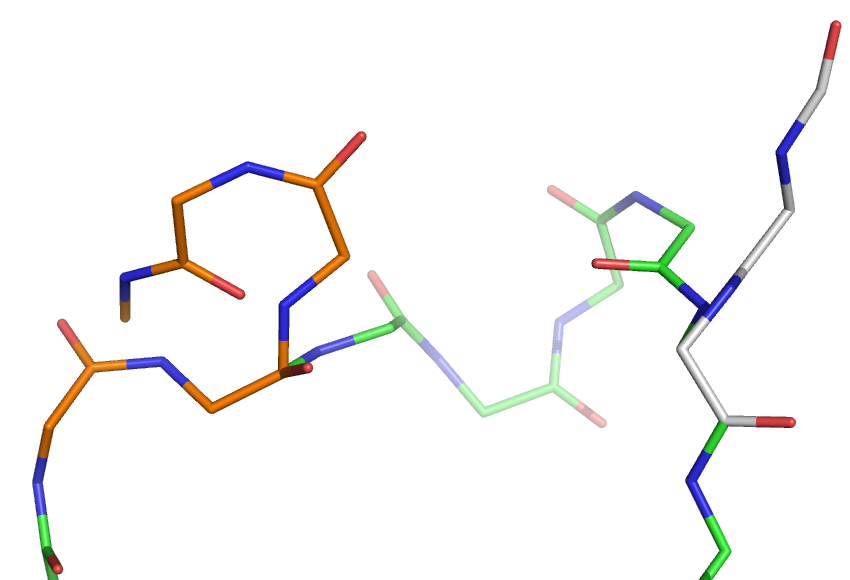
\includegraphics[width=0.52\textwidth]{08-MethodComparison/cloop_fig/stage1.png}}
      \subfigure[Stage 2A: Minimisation of bonded forcefield terms]{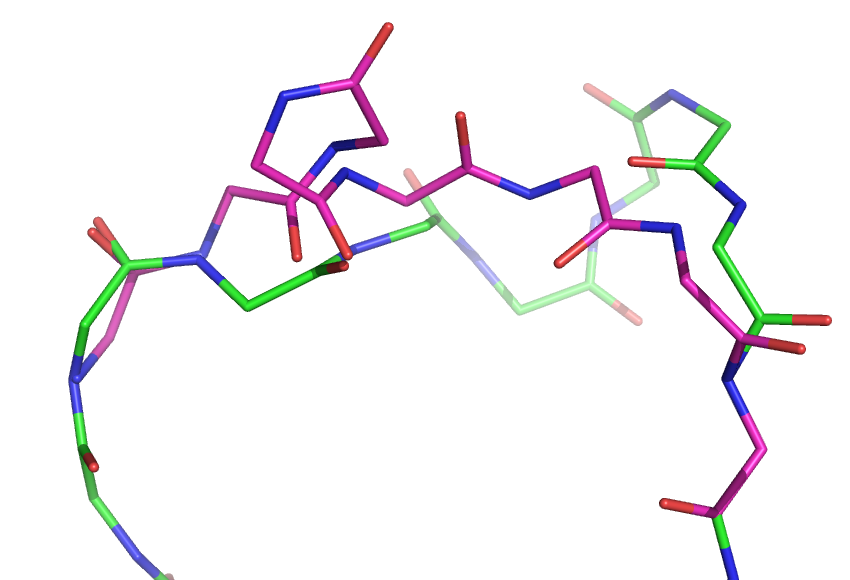
\includegraphics[width=0.52\textwidth]{08-MethodComparison/cloop_fig/stage2a.png}}
      \subfigure[Stage 2B: Minimisation of all \charmm\ energy terms]{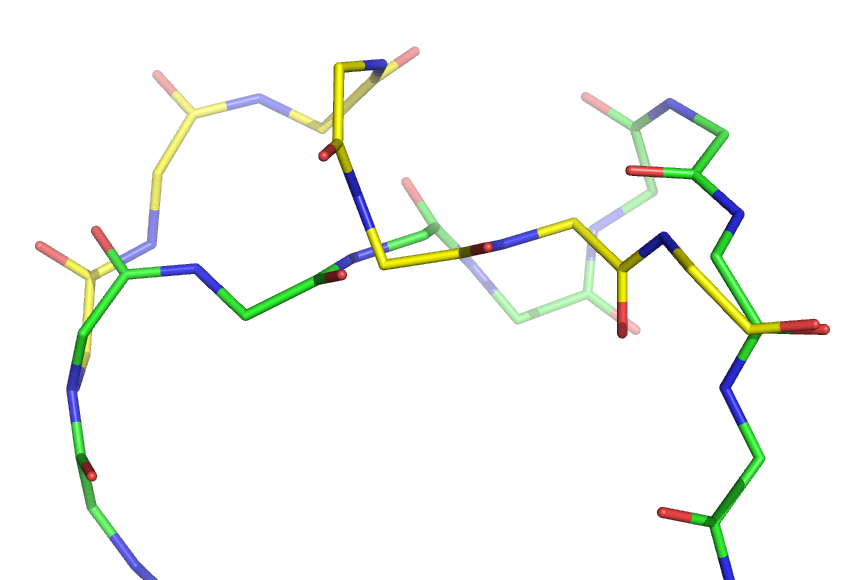
\includegraphics[width=0.52\textwidth]{08-MethodComparison/cloop_fig/stage2b.png}}

    \caption[The individual stages of the \cloop\ build procedure]{The individual stages of the \cloop\ build procedure. In
    all images, the native main-chain conformation is shown in green. \Sidechains\ are present
    at all stages, but omitted for clarity. In
    stage 1, \phipsi\ angles are randomly changed from each anchor to create a new conformation. stage 2A minimises the loop using only bonded-terms and
soft-spheres so that
the atoms can pass within close proximity to each other. It can be seen that the loop structure
in this example, stage 2A clashes with itself. Finally, in stage 2B, a second minimisation occurs using the full \charmm-22 forcefield to generate the final candidate model. This process is repeated until 1,000 models are generated and the lowest energy model selected from these. Figures created using \pymolV.}
    \label{fig:methcomp:cloop}
  \end{center}
\end{figure}

As already mentioned, \cloop\ utilises the \charmm-22 all-atom molecular mechanics forcefield\cite{COMPCHEM:MacKerell1998} for energy assessment of candidate conformations. To improve non-bonded energy calculation efficiency, the BYCC (by-clusters-in-cubes) method\cite{COMPCHEM:Petrella2003} was enabled within \charmm. In addition to the standard energy terms an additional soft-core potential provided by \charmm\ was utilised to smooth non-bonded interactions, specifically the VDW and electrostatic terms. Where the distance between non-bonded atoms falls below a switching distance $r_\mathrm{soft}=0.885$\AA, the soft potential is activated. In the most successful implementation of \cloop, energetic evaluation is performed on the loop and other atoms within a buffer region of 10.0\AA\ surrounding all loop atoms. Each energy minimisation moves only the atoms within the loop itself. It is reported that the buffer region facilitates positive discrimination to more native-like conformations.

The novel minimisation protocol utilised by \cloop\ consists of two stages. The first only considers the bonded-energy of the loop, excluding all non-bonded terms. Under these energetic terms, 200 steps of steepest-descent and then 200 steps of conjugate gradient minimisation were used. An example result of this minimisation is shown 
in figure \ref{fig:methcomp:cloop}b. The second stage enables both the VDW and electrostatic terms. These terms are used for three sequential 100 step minimisations of type steepest-descent, conjugate gradient and Newton-Rhapson respectively; each of which sets the  minimisation threshold to \mbox{0.1 \kcalmol}. An example completed model is illustrated in figure \ref{fig:methcomp:cloop}-c.
The authors report this specific minimisation protocol and energy functions increase loop closure rate substantially, compared to that of a standard \charmm\ minimisation.

Individual candidate models are retained if the final minimised energy is less than \mbox{0.0 \kcalmol}. By default a total of up to 1,000 models are generated. Execution terminates when all 1,000 models are generated or a maximum of 10,000 iterations of the main execution loop have been performed. 
\subsubsection{CLoop Execution}

The original \cloop\ script was subtly modified, to make it more amenable to cluster computation in this work, by adding command-line argument support. The invocation of \cloop\ was then a simple matter of
sending the \charmm\ input script to \charmm\ with small number of command line arguments.
In the example below ``toppar'' refers to the location of the \charmm\ topology definition files and ``xxx'' should be replaced with the appropriate simulation parameters for each job.

\begin{lstlisting}[float, caption={The command line used by the modified \cloop\ script.}, label=listing:methcomp:cloop]
charmm pname=xxx startindex=xxx endindex=xxx toppar=./toppar/ < cloop.inp
\end{lstlisting}


%%%%%%%%%%%%%%%%%%%%%%%%
\subsection{ModLoop}
%%%%%%%%%%%%%%%%%%%%%%%%

\modloop\cite{METHOD:Modloop} is the loop modelling implementation for the comparative modelling application \modeller\ and is also available with an internet interface\cite{METHOD:Modloop_WEB}. In this loop modelling implementation,
the positions of all non-hydrogen atoms of the loop are optimized in the fixed environment of the protein body, with respect to a
pseudo-energy function.\ Multiple energetic optimisations are performed using a mix of conjugate
gradient minimisation combined with molecular dynamics and simulated annealing.
 
The pseudo-energy function, called  \textsc{MolPDF}, uses the bonded forcefield components from the
\charmm-22 \forcefield\ augmented with\ statistical
dihedral angle and non-bonded contact preferences. Dihedral preferences are defined for both \mainchain\ and \sidechain\  torsions. The statistical \phipsi\ potentials were derived per-residue type, from the fitting of a functional
form to the data density of the Ramachandran plot, after it was condensed
onto a 5\degree\ grid.
The non-bonded
contact PMFs are based upon 40 generalised atom types and score in the context of both Cartesian and sequence separations. 
No explicit or implicit solvent or
ligands are included in general, although they could be added in
special cases.

The exact optimisation procedure initially begins from a non-sense  loop conformation; by default merely the individual atoms 
positioned at random
along the vector between the \ca\ atoms of the two anchor residues.
The protocol is defined by two iterations of a simulation cycle, the first
in the absence of the protein body and the second in its presence. The protocol uses two cycles
as it was empirically found that this results in a lower final
energy. Each cycle
begins with up to five 200 step conjugate gradient energy minimisations, each with a successively increasing scaling-factor for the non-bonded energetic terms. This is used in order to relax the non-sense system into a sensible starting conformation. With a low scaling-factor for the non-bonded interactions, the atoms are allowed to pass close to
each other during the minimisation. Next, under MD, simulated annealing is
performed by rapidly heating to 1,000K and then more slowly cooling the system
to 300K. The rate of cooling can be set to one of five settings by the user, the default of which is ``very\_\,fast'' and is used in this work. To achieve a  low
energy end-state, a final conjugate gradient energy minimisation is then performed.

In the original \modloop\ publication, the selected conformation
corresponds to the lowest energy conformation among 500 independent optimizations.
More recent advice from the official on-line \modeller\ support forum suggests that 1,000 models give better results;
which is therefore adopted for this calibration. Additional improvements can be gained by clustering the 1,000 models by structural
similarity and choosing representative members, although this procedure does not appear to be present as part of the standard \modeller\ distribution. 
Following generation of 1,000 viable candidate models based upon \textsc{MolPDF}, a second purely statistical function called \textsc{Dope}\cite{FORCEFIELD:DOPE} (Discrete Optimized Protein Energy) has been shown to have a positive discriminatory effect, in superiority to that of \textsc{MolPDF} in final model selection.
\textsc{Dope} is an atom-distance-dependent statistical potential from a sample of native structures that does not depend on any adjustable parameters.

\subsubsection{A Python Script to Launch ModLoop }

Listing \ref{listing:methcomp:modloop} illustrates the Python script which is used to instruct the \modeller\ application to build a single loop structure. Listing \ref{listing:methcomp:modloop_dope} then goes on to show how \textsc{Dope} scores are generated for the 1,000 models produced by the first script.

\lstset{language=Python}
\begin{lstlisting}[float, caption={\modloop\ main\ Python launch script.}, label=listing:methcomp:modloop]

from modeller.automodel import *

log.verbose()
env = environ()

env.io.atom_files_directory = './'
env.io.output_directory = './'

class myloop(loopmodel):
    def select_loop_atoms(self):
        self.pick_atoms(selection_segment=('100:A', '107:A'), selection_status='INITIALIZE')

m = myloop(env,
           inimodel='1AUN_.min.pdb',
           sequence='1AUN__100_8')

m.loop.starting_model = 1
m.loop.ending_model  = 1000
m.loop.md_level = refine.very_fast

m.make()
\end{lstlisting}


\begin{lstlisting}[float, caption={The \modloop\ Python script used to generate \textsc{Dope} scores.}, label=listing:methcomp:modloop_dope]
from sys import *
from array import array
from modeller import *
from modeller.scripts import *
        
modelCount = 1000
stem = argv[1]

env = environ()
env.libs.topology.read(file='$(LIB)/top_heav.lib')
env.libs.parameters.read(file='$(LIB)/par.lib')

data = array('f')

for i in range(modelCount):

        fileName = stem + "\\" + stem + ".BL"   
        num  = i+1 
        if num < 1000:
                fileName += '0'
        if num < 100:
                fileName += '0'
        if num < 10:
                fileName += '0'    

        fileName += str(num) + "0001.pdb"
                
        mdl = model(env)
        mdl.read(file=fileName)
        aln = alignment(env)
        code = stem
        
        # generate topology
        aln.append_model(mdl, atom_files=fileName, align_codes=code)
        aln.append_model(mdl, atom_files=fileName, align_codes=code+'-ini')
        mdl.generate_topology(aln, sequence=code+'-ini')
        mdl.transfer_xyz(aln)
        
        dopeScore = mdl.assess_dope()

        data.append( dopeScore )
            
filename = stem + ".dope"       
FILE = open(filename,"w")     
for i in range(0, modelCount):
    FILE.writelines( str(i+1) + ' ' + str(data[i]) + '\n')
FILE.close()
\end{lstlisting}







%%%%%%%%%%%%%%%%%%%%%%%%
\subsection{Orchestrar}
\label{section:methcomp:orchestrar}
%%%%%%%%%%%%%%%%%%%%%%%%


\textsc{Orchestrar} is the name for a group of applications from the Cambridge crystallography and bioinformatics 
 group intended as a complete comparative modelling suite. Here, we focus on three published applications which select
loop fragments from databases: \textsc{Fread}\cite{METHOD:CODA}, \textsc{Petra}\cite{METHOD:Petra} and \textsc{Coda}\cite{METHOD:CODA} which are knowledge-based, \abinitio\ and consensus methods respectively. Additional supplementary applications are supplied to build complete protein models.
In total, \emph{eight} separate applications are required to re-construct a surface
loop onto a protein scaffold.


\subsubsection{Petra}

\textsc{Petra} is the published name of an algorithm for selecting loop fragments from an \abinitio\ polypeptide fragment database, termed the APD, with the aim of their subsequent use in protein loop modelling. 

The APD itself represents all viable polypeptide fragments of up to 12 residues in length, which lack self-clashes, generated by the enumeration of a set of 8 parametised \phipsi\ pairs. This gives $1.0 \times 10^8$ valid fragments from a total of $8.12 \times 10^8$ possible permutations. The  8 parametised \phipsi\ pairs were derived iteratively from their ability to represent a trial set of structures. Due to the storage implications,
only the \phipsi\ identifiers and four \ca\ separations are stored for use in fragment selection, rather than structural coordinates. Although \mer{12} fragments are stored
within the APD,
in order to connect them to the protein body, four anchor residues are required
and therefore only loops of up to eight residues in length can be modelled,
as shown in figure \ref{fig:methcomp:petrafrag}.

\begin{figure}[hp]
\begin{center}
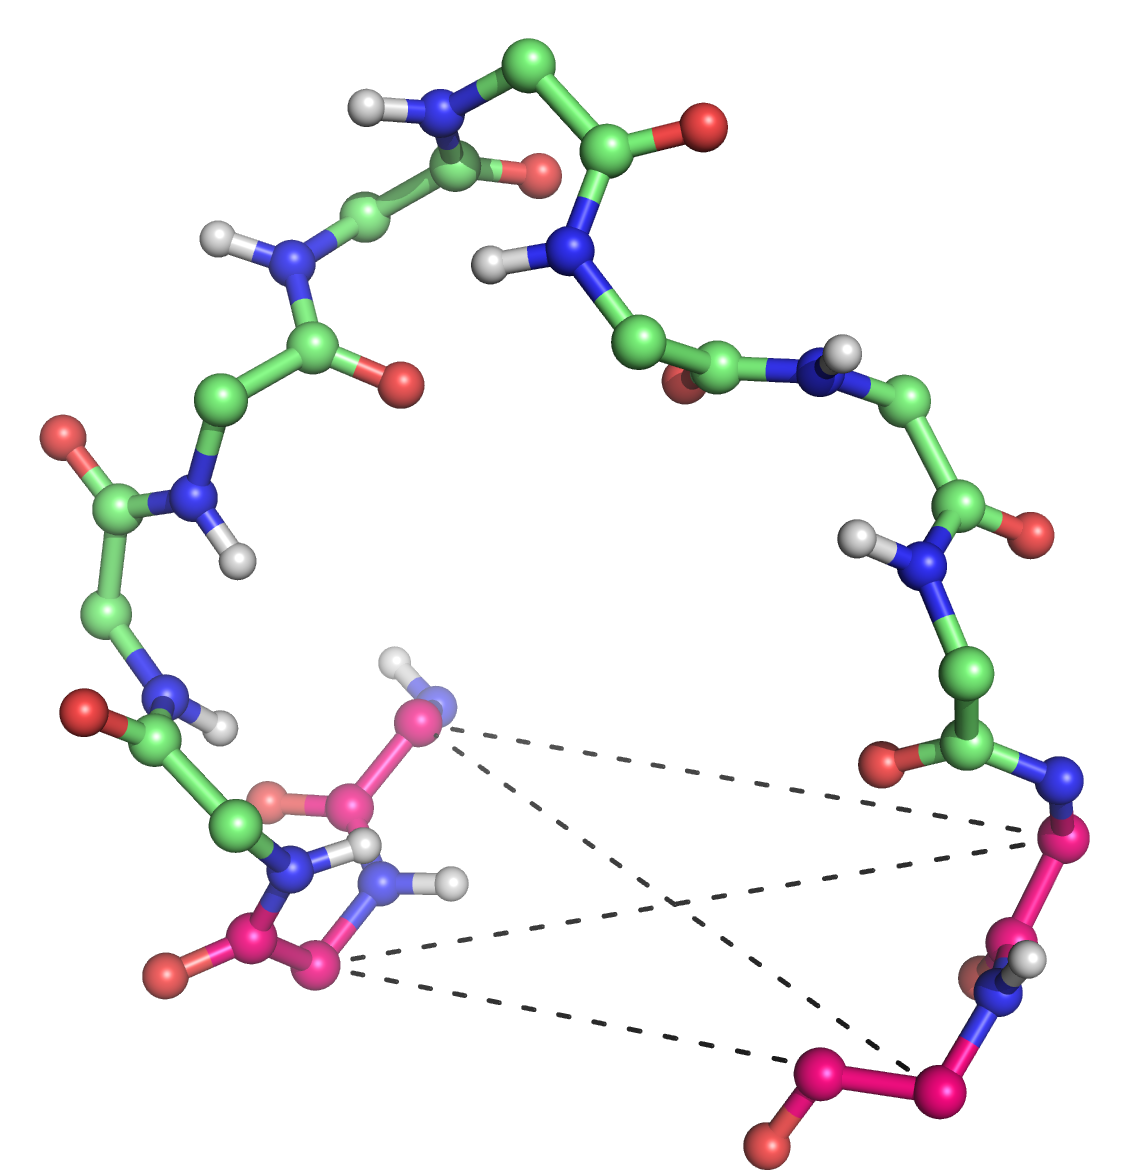
\includegraphics[width=0.6\textwidth]{./08-MethodComparison/petra/1A73A_97_12.png}
\caption[A Petra fragment]{An example \textsc{Petra} fragment: An example maximum-length \mer{12} fragment is shown. The four anchor-residues and the \mer{8} loop itself are shown in magenta and green
respectively. The four \ca\ separations, used during modelling to determine if a loop can bridge the gap between a given pair of anchor residues, are shown as
dashed lines.}
\label{fig:methcomp:petrafrag}
\end{center}
\end{figure}



It is claimed that 96\% of \mer{5} fragments, in \xray\ structures of \textless$1.5$\AA\ resolution and \textless25\% pairwise identity, have a  1.0\AA\ RMSD structure within the database. This score is however, not ideal as it includes regular secondary structure, which by definition has tightly defined \phipsi\ properties. A more robust score would look solely at native loop fragments and would also comment on longer loop lengths.

In terms of the implementation, \textsc{Petra} is a pair of applications within \textsc{Orchestrar} called \textsc{Read7} and \textsc{Minus2}. \textsc{Read7} is solely designed to reduce the number of conformations that pass into \textsc{Minus2} by using a set of three primary rule-based filters.
The three, successively more expensive, rule-based filters are applied in turn. The first filter, illustrated in figure \ref{fig:methcomp:petrafrag},
involves matching the four \ca\ atomic separations
to those of the anchor residues of the protein body. The second scores the propensity of
the loop sequence for the \phipsi\ angles in the chosen loop fragment. Finally,
filtering occurs based on the RMSD measured following superimposition of the \mainchain\ atoms of the
four fragment anchor residues to the corresponding residues in the protein body. The fragments are then sorted by this RMSD.

Any fragments which pass these filters are sent to \textsc{Minus2} where they are scored by $E_K$. This scoring function is the same all-atom distance-dependent conditional probability
function, developed by Samudrala and Moult, that is also used by \rapper\cite{FORCEFIELD:Samudrala1998} (discussed in section \ref{section:methcomp:rapper_intro}). The calculation
scores the loop atoms in the context of the protein body, ignoring the first and last residues of the fragment. The sorted fragment list is traversed until ten structures are found that fall below the cut-off value for $E_K$ or until the list is exhausted.
In the published work, $E_K$ is shown to have discriminatory power against
poor loop candidates, but lacks in the ability to discriminate against non-native-like
fragments. A typical distribution is shown in figure \ref{fig:methcomp:petraekdist}.

\begin{figure}[hp]
\begin{center}
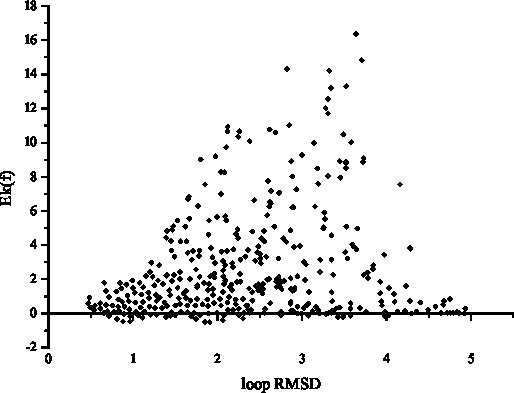
\includegraphics[width=0.7\textwidth]{./08-MethodComparison/petra/ek_vs_rmsd.pdf}
\caption[Typical $E_k(F)$ versus RMSD distribution.]{A typical $E_k(F)$ versus RMSD distribution. Data from\cite{METHOD:Petra}. The distribution shows poor discrimination towards native-like states, but can be used to effectively filter against some types of non-native structures.}
\label{fig:methcomp:petraekdist}
\end{center}
\end{figure}

\subsubsection{Fread}
The primary \textsc{Fread} database, F20\cite{METHOD:FREAD:F20}, contains around 5,000 structures obtained from structures of $<$2.0\AA\ resolution within the \textsc{Homstrad} database\cite{SEQUENCE:HOMSTRAD}. \fread\ selects fragments using four rule-based filters:

\begin{itemize} \isep
\item 
$D_c(F)$: The \ca\ separation of the target and fragment anchors
\item
$S_c(F)$: The score using environmentally-constrained sequence substitution tables
\item
$R(F)$: The RMSD of the target and fragment \mainchain\ anchor atoms
\item
$E_k(F)$: The energy of the fragment within the target structure
\end{itemize}

Initially, $D_c(F)$ and $S_c(F)$ are used to pre-screen structural fragments from the database. Structures which pass these two pre-filters are then sorted
by $R(F)$. Finally, up to 10 fragments are selected which are above a cut-off
value for $E_k(F)$. The default chosen cut-off is dependent on the length of the loop, however, it can be altered to change the coverage of conformational
space.

Environmentally-constrained substitution tables were found to have a strong
discriminatory effect where sequence identity was high, showing that residues
with similar chemical identity and structural context are more likely to adopt similar overall structures.
With sequences of low identity, it was found that the tables had significantly
less effect, but were still of benefit in filtering against highly improbable
candidate fragments.


In terms of performance, \textsc{Fread} was found to perform significantly better  when the best top 10 scored fragments were considered as opposed to the single best. More than 10 fragments were found to provide little additional coverage. This further illustrates that the scoring function is capable of selecting some native-like fragments, but the final discrimination between the best candidates is, not surprisingly, imperfect.

\subsubsection{Coda}
\label{section:methcomp:coda}
For each of the fragments selected by \textsc{Fread} and \textsc{Petra},
\coda\ considers all possible pairings. These pairings are then filtered by a large range of different scores. These include the \phipsi\ difference between the fragment pair; the sum of the  original $E_k(F)$
evaluations; the RMSD between the fragments following superimposition on the protein core anchor residues ($E_d$); the sum of their ranks ($H_p$); and finally, the filter scores from the original
\textsc{Fread} and \textsc{Petra} output. All these filters must be under given cutoffs, originally optimised for maximal data coverage by \emph{another} separate stand-alone application.

Once a pair is selected, \coda\ must then choose between the \textsc{Fread} and \textsc{Petra} fragments. The sum of $E_k(F)$ was found to be a very
weak indicator for selection except for very specific cases in
which it removed false positives.
 It was also found that if \textsc{Fread}s $S_c(F)$
was very good, then the fragment from \textsc{Fread} was generally most native-like. In general, it is usual
for the empirical filters used in \coda\
to select the \textsc{Petra} prediction for
lengths six to eight and the \textsc{Fread} prediction for shorter lengths.
Final conclusions showed that the consensus found by \textsc{Coda} did indeed improve over the
results for the individual programs. The standard
deviation of the results also dropped indicating a more
consistent predictive ability than that shown by \textsc{Petra} and
\textsc{Fread} individually.
  

\subsubsection{Orchestrar Work-flow}

In brief summary, the roles of the eight required applications are as follows. Each application in turn uses the output files of the pervious application for its input along with various documented command-line parameters. To begin, \textsc{Joy}\cite{SEQUENCE:JOY} is executed to produce a sequence alignment of the protein to itself, solely to create prerequisite input files for the following applications. In full comparative modelling a divergent sequence would be used at this stage and further steps added, in order to remodel the protein core. \textsc{Petra} itself is split into two applications called \textsc{Read7} and \textsc{Minus2}, the first of which selects fragments from the APD and the second of which selects within that subset. The sister application  \textsc{Fread} then performs an analogous function on the F20 database of PDB-derived fragments. Valid fragments from these two applications can then be collated, paired and the most suitable chosen by \coda. As the fragment databases do not store \sidechain\ conformations, at this stage a backbone-only polypeptide  fragment of the same length of the loop plus two additional residues at either end, has been chosen. The fragment has been reoriented so that these anchor residues overlay with the two anchors of the protein body in Cartesian space. Two applications called \textsc{Pre-Tuner} and \textsc{Tuner} are then used to merge this fragment onto the body of the protein to produce a backbone only model. Finally, \textsc{Andante}\cite{METHOD:ANDANTE} is called to re-build all \sidechains\ on to the protein backbone and model loop, producing the final model.

\subsubsection{Launching Orchestrar}

For this comparison, \textsc{Orchestrar} was launched with a custom made shell-script in the following format. Some environment variable declarations and code-lines for intermediate-file clean-up are omitted for clarity.

\begin{lstlisting}[float, caption={An excerpt from the launch script created for \textsc{Orchestrar} during this work.}, label=listing:methcomp:orchestrar]
# Command-line arguments
echo Stem: $1
echo StartRes: $2
echo Length: $3
stem=$1_$2_$3

# Sequence Generation
echo Running 'Joy':
$JBIN/joy $1.ali

# Loop Selection
echo Running 'Fread':
$JBIN/FREAD3 -pdb $1.min.pdb -seq $1.ali -startres $2 -len $3 -o $stem.fread
echo Running 'Read7':
$JBIN/Read7 -pdb $1.min.pdb -seq $1.ali -startres $2 -len $3 -o $stem.read7
echo Running 'Minus':
$JBIN/MINUS2 -pdb $1.min.pdb -seq $1.ali -startres $2 -len $3 -o $stem.petra -m $stem.read7

# Stitch loop allowing DB information
echo Running 'Coda_DB':
$JBIN/CODA3 -ff $stem.fread -mf $stem.petra -o $stem.both.coda -len $3
echo Running 'PyConcat_DB':
python $JBIN/concat_coda.py $1 $stem | $JBIN/pretuner > $stem.coda.meld
echo Running 'Tuner_DB':
$JBIN/tuner -pdb $stem.coda.meld -out $stem.coda.tuner -meld -dino 
echo Running 'Andante_DB':
$JBIN/andante -i $1 -cm $stem.coda.tuner -chi1 -chi12 -minpid 40 -minb 40
              -ccc 7.0 -cbb 10.0 -o $stem.coda.pdb

# Stitch loop NOT allowing DB information - i.e. petra only
echo Running 'Coda_AbInitio':
$JBIN/CODA3 -up -ty 3 -ff $stem.fread -mf $stem.petra -o $stem.petra.coda -len $3
echo Running 'PyConcat_AbInitio':
python $JBIN/concat_petra.py $1 $stem | $JBIN/pretuner > $stem.petra.meld 
echo Running 'Tuner_AbInitio':
$JBIN/tuner -pdb $stem.petra.meld -out $stem.petra.tuner -meld -dino 
echo Running 'Andante_AbInitio':
$JBIN/andante -i $1 -cm $stem.petra.tuner -chi1 -chi12 -minpid 40 -minb 40
              -ccc 7.0 -cbb 10.0 -o $stem.petra.pdb
              
\end{lstlisting}



%%%%%%%%%%%%%%%%%%
\subsection{PLOP}
%%%%%%%%%%%%%%%%%%

\plop, or Protein Local Optimization Program, is a single application by UCSF (University of California, San Francisco), for protein modelling using all-atom energy functions. Functionality includes multi-scale truncated Newton-Rhapson minimisation protocol, \sidechain\ optimization\cite{METHOD:Plop:Jacobson2002A,METHOD:Plop:Jacobson2002B}, loop prediction\cite{METHOD:Plop} and the prediction of helix positions and orientations\cite{METHOD:Plop:Xin2004}. The performance of the loop prediction methodology is tested in this work. 

The three-tier loop modelling methodology utilises  hierarchical build-up, clustering techniques and side-chain optimisation in order to reduce the magnitude of conformational space that must be explored.
The initial stage of the process is a loop backbone build-up from both anchor residues, termed the left and right branches. Build-up is performed from a restrained \phipsi\ angle library derived from a non-redundant subset of $>$500 \xray\ structures at $<$2.2\AA\ resolution. The library was generated by dividing the Ramachandran plot into a 5\degree\ grid, where each square was only included if it contained more than 5 examples within the PDB subset. The resulting high-resolution library contained 747, 215 and 866 \phipsi\ pairs for Glycine, Proline and all other amino acids respectively. The conformational space of such a library is so vast that any exhaustive search is impossible and thus requires a sampling procedure. The authors comment that such a large library is required to prevent ``discretisation errors'' from fundamentally limiting the conformational search procedure. For each residue position all of these states are screened by four filters described below. The resultant candidates are then further reduced in number by retaining a subset in which all pairs obey the relationship $\Phi^{2}+\Psi^{2}<R^{2}_\mathrm{eff}$, where $R_\mathrm{eff}$ is effectively a linear distance on a Ramachandran plot. 

During build-up four basic filters are used to reduce the number of candidates. Firstly, candidates are excluded where there is a steric clash, scored by the ratio of the distance between the atom centres and the sum of the atom VDW radii being less than 0.7. Secondly, for each loop residue all possible \sidechain\ rotamers from a 30\degree\ library are built and sterically screened until one is found which does not contact atoms in the protein body. This ensures that there is sufficient space to pack each \sidechain. The atoms in the loop are not considered, leaving the possibility that there may be no valid conformation that avoids the loop clashing with itself. Thirdly, loop conformations are rejected if they cause the loop to extend away from the protein body. In 500 test cases they showed that 99\% of distances from \ca-atoms to all other protein atoms are $<$6.32\AA. This constraint is then used to filter candidates. Finally, empirical distances between loop and anchor \ca\ centres are used to ensure that the loop conformation can span each remaining spatial gap. In addition to the four standard constraints, user defined Cartesian and torsional restraints can be optionally applied.

Following build-up a set of conformations extending from the left and right branches must be searched to find all pairs which are in $<$0.5\AA\ contact at the central join. For each pair the \ca\ positions are averaged and the \sidechain\  atoms rebuilt using standard geometry. These joined conformations are then further screened. Firstly, the  N--\ca--C angle at the join must be within 25\degree\ of its 111.1\degree\ optimal. Secondly the \phipsi\ torsions of the closure residue must fall within 25\degree\ of the allowed regions of the Ramachandran map. Thirdly there must be no steric clashes between atoms within the closed loop. Finally the rotamer library is scanned to ensure there is at least one sterically valid rotamer for the closure residue.

It is noted by the authors that sampling should be dependent on the inherent flexibility of the loop; the more flexible a loop, the more viable conformations will be present at this stage and there is a wide variation. It is also noted that there is a correlation between loop flexibility, anchor separation and loop glycine and proline content. \plop, therefore, caps the maximum number of loops at $10^6$ due to speed and memory considerations. A minimum is defined as $2^N$ where N is the number of loop residues. The sampling resolution is then decreased until the number of candidates lie within acceptable bounds. Clustering on the set of closed loop conformations can then be performed.

All structures that are present at this stage have no steric clashes and have not been optimised. The clustering is performed using a K-means algorithm\cite{COMPCHEM:KMeans} and selects a representative set of loop candidates to optimise and score. The algorithm scales linearly with number of candidates, but cannot guarantee reaching the globally optimal solution. The number of clusters in the algorithm must be determined in advance and is set empirically to be four times the loop length. The criterion used for similarity was the Cartesian \crms\ of the N, \ca, \cb, and C atoms of each residue. If large clusters with high variance emerge, they are split once and clustering is repeated. Cluster representatives for optimisation are chosen from each cluster, preferentially selecting those with low distance to the cluster centre. 

\Sidechain\ optimisation\cite{METHOD:Plop:Jacobson2002A} is performed on the resulting structures using a 10\degree\ rotamer library. For computational efficiency the library is first screened by hard-sphere overlap prior to ranking on the detailed forcefield. Iterative\ optimisation is performed by sequentially changing each \sidechain\ to its optimum rotamer until convergence occurs. 

Finally, a full Cartesian minimisation is performed on the final loop. The multi-scale minimisation algorithm used is based on the TNPACK implementation\cite{METHOD:MINIM:Xie1999,METHOD:MINIM:Schlick1987,METHOD:MINIM:Schlick1992} of the truncated Newton-Rhapson method. In this the short-range and long-range energetic components are segregated. The \forcefield\ used for the simulation was the all-atom \opls\cite{COMPCHEM:OPLS,COMPCHEM:OPLS:B} forcefield with solvation free energy estimated using a Surface Generalised Born (SGB) with a non-polar estimator\cite{FORCEFIELD:SGB:NP}. Correction terms were used to improve the correlation between SGB and the Poisson-Boltzmann calculations\cite{FORCEFIELD:SGB}.

\subsubsection{Plop Launch Script}

For this comparison, \plop\ was launched with an generated script in the following format.

\begin{lstlisting}[caption={The \plop\ launch script: job\_\,name.inp.}, label=listing:methcomp:plop] 
data /shared_mount/plop/data/
job job_name
load pdb job_name.db.pdb seqres yes opt yes
loop predict A:20 A:26
pdbfile job_name.pdb
rmsdfile job_name.rmsd
\end{lstlisting}


%%%%%%%%%%%%%%%%%%%
\subsection{Rapper}
\label{section:methcomp:rapper_intro}
%%%%%%%%%%%%%%%%%%% 

The \rapper\ modelling process fundamentally comprises  the \rapper\ search method\cite{METHOD:RapperB} and the  \textsc{Rapdf} all-atom statistical potential\cite{METHOD:RapperA}.

\subsubsection{The Rapper Conformational Search}

Originally devised as a whole protein prediction system, \rapper\ was adapted to confront the loop modelling problem. It is based on a backbone torsion build-up method, using fixed bond lengths and angles, which progresses from the N-terminal
end of the loop conformation. The \rapper\ conformational search focuses on the generation of \mainchain\
conformations, \ie the positions of the \bbatoms\ and additionally in this
case the \cb\ atom. Each generated structure fulfills the stereochemical requirements of idealised geometry, favourable \phipsi\ angles and excluded volume. Atoms are represented as hard-spheres with van der
Waals radii reduced by 20\% to ensure that only energetically unfeasible conformations are rejected by the hard-spheres excluded-volume
restraint.

The \phipsi\ set is fine-grained in nature. The authors concluded that this
is superior to a simple exhaustive enumeration from a coarse-gained set. Residue-specific, propensity-weighted state sets, generated on a 5\degree\
grid over the Ramachandran map yielded up to $72^{2}$ states per residue.
The exact counts are listed in table \ref{table:methcomp:rapperstates}.
The Ramachandran data was derived from all residue \phipsi\ data within the Top500 database of protein structures\footnote{http://kinemage.biochem.duke.edu/databases/top500.php}.
The \rapper\ search method completely neglects the 0\degree\ cis state for
the \Omg \ backbone torsion.

\begin{table}[hptb]
\begin{center}
\begin{tabular}{+l^c^c^l^l^c^c}
\toprule
\rowstyle{\bfseries}
  Amino Acid & States & \% & \qquad & Amino Acid & States & \%\\
\midrule

Glycine        & 4,264  &  82.3   &&   Glutamine      & 2,573  &  49.6  \\
Aspartic Acid  & 3,275  &  63.2   &&   Cysteine       & 2,541  &  49.0  \\
Serine         & 3,203  &  61.8   &&   Phenylalanine  & 2,523  &  48.7  \\
Asparagine     & 3,082  &  59.5   &&   Tyrosine       & 2,497  &  48.2  \\
Alanine        & 3,055  &  58.9   &&   Glutamic Acid  & 2,491  &  48.1  \\
Threonine      & 2,870  &  55.4   &&   Valine         & 2,403  &  46.4  \\
Histidine      & 2,748  &  53.0   &&   Methionine     & 2,268  &  43.8  \\
Leucine        & 2,737  &  52.8   &&   Tryptophan     & 2,257  &  43.5  \\
Lysine         & 2,658  &  51.3   &&   Isoleucine     & 2,229  &  43.0  \\
Arginine       & 2,582  &  49.8   &&   Proline        & 1,207  &  23.3  \\


\bottomrule

\end{tabular}
\caption[\rapper\ per-residue-type \phipsi\ states]{\rapper\ per-residue-type \phipsi\ states. The \% values are quoted in reference to the maximum count of $72^2$, based on a complete 5\degree\ grid.}
\label{table:methcomp:rapperstates}
\end{center}
\end{table}

Conformational sampling occurs using a ``scheduling algorithm'' which attempts to distribute the search fairly between the torsional states.
The algorithm begins with the allocation of a fixed-length queue of zero-length loop conformations. At each step of
the process, a conformation is taken from the front of the queue and extended by
a single residue. The extension occurs using a random selection from the
\phipsi\ angle set. Up to 25 \phipsi\ pairs are attempted before either a conformation
is found that passes all geometric tests, or the whole conformation
is discarded. If a conformation is found which passes, both the extended
and unextended versions are added to the back of the queue. This process
continues until 1,000 conformations are completed of the full loop length
plus one dummy anchor-residue. For each conformation to survive, it must satisfy all restraints, bridge the gap to the C-terminal anchor and not share \textless0.2\AA\  \crms\ similarity with any other accepted conformation.

During the build process, it is assured that closure is ultimately possible by measuring
the distance between the \ca\ of the current end of the growing loop and
the \ca\ of the  C-terminal anchor residue ($d$), by the formula $d <\ 3.8(n-i+1)+1$\AA.
The final 1\AA\ is required to allow some deviation of the loop and C-terminal
anchor residues, which are ultimately closed using a dihedral angle minimisation
with a harmonic potential between the respective N and \ca\ atoms. The minimiser iteratively perturbs a randomly chosen $\Phi$ or $\Psi$ angle by a random value, taken from a uniform distribution
of $\pm 5.0$\degree. The perturbation is accepted if the new
\phipsi\ state has non-zero propensity, the excluded-volume
restraint is satisfied and C-terminal overlap improves. The minimization
continues until 10,000 steps have been made or the average C-terminal overlap
over the previous 50 steps drops below a threshold. 

Following the definition of the \mainchain\ conformations, \sidechains\ are added using \textsc{Scwrl}\cite{METHOD:SCWRL_1} in the context of the entire protein. \textsc{Scwrl} relies upon an graph-theory based algorithm to select the most favorable rotamers for each loop residue from a backbone-dependent rotamer library. During this refinement
process, all steric clashes between modelled \sidechains\
and the rest of the structure are resolved.

Following generation of the 1,000 viable conformations, discrimination between them
is performed using the \textsc{Rapdf} potential described in the following
section. In the original complementary work\cite{METHOD:RapperA}, the discriminatory
power of \textsc{Amber/Gbsa} was also assessed.
 
\subsubsection{The RAPDF All-atom Statistical Potential}

Following generation of large ensembles of closed conformations from the \rapper\ conformational search method which satisfied geometric considerations,
the \textsc{Rapdf} potential is used to select candidates. The \textsc{Rapdf} potential itself is a probability discrimination function
based on a statistical Bayesian formulation, originally developed by Samudrala and Moult\cite{FORCEFIELD:Samudrala1998}. In this formulation, all heavy-atoms in all residue-types are defined independently, resulting in a total of 167 atom-types. For all possible pairs of atom-types, interaction scores were derived from a non-redundant protein structure database, separated into 18 discrete distance bins. Importantly, no distinction is made between local and non-local interactions. The authors of this work report that this does not diminish decoy discrimination power, however other work has concluded that such interactions are highly important\cite{COMPCHEM:Zha2004}.

In the original
work, 50 loop candidates were minimised using \textsc{Amber/Gbsa}.
Importantly, even though the internet-based version of \rapper\ provides this option, it does not appear to be available in the distributed version of the application. It  is, therefore, not presented in the results section of this critical method comparison.

Some  important conclusions were drawn in relation to forcefield discrimination:\begin{itemize}\isep

\item 
Unsurprisingly, the authors conclude that the quality of anchor superimposition alone is a poor score for the discrimination of native and non-native conformations.
Interestingly, they also conclude that the \textsc{Rapdf} function is not
significantly better.

\item
The \amber\ \gbsa\ energy function has better correlation with \crms\ to native than the \textsc{Rapdf}. In fact, a dramatic
improvement in selection accuracy was observed at
longer loop lengths when scoring with the \amber\ \gbsa\ \forcefield.
\item
\amber\ \gbsa\ minimised fragments
had, on average, consistently lower \crms\ values
(by 0.1\AA) than their initial conformations, unless the initial
conformations were far away from the native structure.

\item
There are significant numbers of cases where the \amber\ gas-phase
minimisation selects conformers of lower \crms\ than the \amber\ \gbsa\ minimisation.
This suggests difficulties in the underlying solvent model.
\end{itemize}

\subsubsection{Rapper Execution}

For this method calibration, as directed by available documentation, \rapper\ was initiated with the following runtime execution flags, where $x$ and $y$ are first and last residue indices of the loop.

\begin{lstlisting}[caption={The command-line used for \rapper\ execution.}, label=listing:methcomp:rapper]
rapper -models 1000 -pdb job_name.pdb -start x -stop y -sidechain-mode smart
\end{lstlisting} 






%%%%%%%%%%%%%%%%%%%%%%%%%%%%%%%
\section{The Comparison Format}
\label{section:methcomp:comparison_format}
%%%%%%%%%%%%%%%%%%%%%%%%%%%%%%%

For each candidate loop, each of the selected applications was
executed and its best predictions generated. For
each method the prediction with the single best
score was obtained and compared to the minimised \xray\ structure from \thothloopdb\ using the method
described in section \ref{section:methcomp:superimpos}. The statistical
distribution of the success of each method across the entire database was
then analysed and is reported in section \ref{section:methcomp:results}. 
\subsection{Application Parameter Space}

For each of the methods used in this study, there are a number of options, settings and parameters that are exposed for the user to customise the behaviour
of the modelling process. For reasons of fairness, simplicity and to prevent an explosion in parameter space during the analysis, only the default settings for each application were used during the comparison. In cases where publicly available documentation recommended that alternative settings produced better results, these were used in preference. Specific changes are discussed in more detail where appropriate.

   

\subsection{Scoring Method Effectiveness}
\label{section:methcomp:superimpos}



Following structural superimposition, it is usual to quote \crms\ values as the measure of structural deviation. This is calculated using equation \ref{eq:method:rmsd},  where $\vec r_i(A)$ is the Cartesian coordinate of atom $i$ in structure $A$, which is
measured against the equivalent atom in structure $B$. From this equation, a low
\crms\ value indicates
good structural similarity.

\begin{equation}
d_\mathrm{rms}=\sqrt{\frac{1}{N_\mathrm{atoms}} \displaystyle\sum_{i=1}^\mathrm{N_\mathrm{atoms}} \left\vert \vec r_i(A)-\vec r_i(B)\right\vert^2 }
\label{eq:method:rmsd}
\end{equation}

Previous individual publications have reported results using a variety of different measures of effectiveness. Most comparisons utilise superimposition, but often differ in precisely which sections of the completed model are superimposed on the crystal structure and which atoms are used in any RMSD calculations. It is usual to calculate the optimal superimposition of either \ca\ or backbone atom\ coordinates, however sometimes all heavy atoms are used.

Some calibrations involve superimposition of just the generated loop structure itself onto the corresponding native fragment\cite{METHOD:LIP}.  This technique often reports  low \crms\ values which are unrepresentative
with regard to the viability of the model loop structure in its \emph{native context}. If
these unrepresentative low-\crms\, structures are overlaid on the native structure, they either do not allow contact of the loop termini with their respective anchor residues or would exhibit \cacbvects\ of incorrect orientation compared to the native. Loop models, which are used to assess structural or functional significance and biological or pharmaceutical interactions, must be evaluated with respect to the protein body in order to allow interpretation at atomic resolution.
The conclusion, therefore, is that superimposition methods that yield no information about the comparative orientation of the loop model with respect to the protein body are not appropriate. 

Other assessments superimpose the complete protein model with that of the crystal structure\cite{METHOD:Plop}. Whilst the orientation of the loop with respect to its anchors is ensured in this comparison, larger deviations in loop atom positions can be compensated for via small deviations over the entire protein rigid-body. As all the deviations are small, they contribute little to the \crms, however they can dramatically reduce the penalty from larger deviations in the loop structure itself. It is,  therefore, the view of the author that the most representative method is to perfectly superimpose \emph{only}  non-loop atoms  and measure deviation in the position of \emph{loop atoms} only.

There are multiple measures of structural deviation. In this study three independent measures are quoted. The first is Cartesian coordinate deviation of all heavy \mainchain\ atoms -- namely the \bbatoms\ -- which gives a measure of correct absolute backbone placement. However, with this measure it is possible to get low \crms\ structures which are non-native-like. An example of this would be a complementary set of torsional $\sim$180\degree\ inversions that allowed the backbone to assume a native-like path in space, but utilising non-native  \mainchain\ torsions. In view of this, in addition to the Cartesian measure, backbone torsional deviation is also reported over the \phipsiomg\ backbone torsions, defined by equation \ref{eq:method:torsional_rmsd}.
The prime symbols denote the equivalent torsion in the reference state.

\begin{equation}
\mathrm{\arms}=\sqrt{\frac{1}{N_\mathrm{residues}}\displaystyle\sum_{i=1}^{N_\mathrm{residues}}
\left( \Phi_i-\Phi'_i  \right)^2
+ \left( \Psi_i-\Psi'_i \right)^2 
+ \left( \Omega_i-\Omega'_i \right)^2   
}
\label{eq:method:torsional_rmsd}
\end{equation}

The final measure of all-heavy-atom Cartesian \crms\ takes absolute \sidechain\ placement into account, with the caveat that this score only valid in the context of correct backbone assignment, as otherwise (by definition) any \sidechains\ will certainly be in the incorrect orientation.
With all these measurements any  significant backbone deviations will result
in
 large \crms\ outliers. In order to describe the impact of high \crms\  predictions the median
average is reported in addition to the mean.



\subsection{Choosing a Prediction}

Most of the methods in this work produce a significant amount of structural
data following execution. Methods such as \plop\ and \rapper\ output only
structures which are deemed to be of high quality. Other methods such as
\cloop\ and \modloop\ output a requested fixed number of refined structures regardless
of the quality, although each candidate is a viable closed loop conformation. Each structure is associated with a score, which
represents the methods' view of how native-like the prediction is.  

In some loop modelling publications some authors quote the best
\crms\ reached for a given simulation with no regard for the scores associated
with those predictions\cite{METHOD:CLOOP}. In a real blind-test, of course, one has no idea what the \crms\ value is for a selection of 1,000 predictions and therefore such a score is only of use during calibration. It is, therefore, far more interesting to know which structure would be chosen by an end-user of each
method as the most likely to be native-like.
In this work, the structure with the single best associated score is extracted for use in the statistical analysis. 









%%%%%%%%%%%%%%%%%
\section{Results}
\label{section:methcomp:results}
%%%%%%%%%%%%%%%%%


During the analysis of the structural data produced during this study, a number of different statistical quantities were measured for each of the three chosen scoring criteria of prediction quality defined previously in section \ref{section:methcomp:superimpos} -- \mainchain\ atom \crms, heavy-atom \crms\ and torsional RMSD. Each of these were measured per prediction-method and loop-length providing  a total of $3\times8\times6=144$ histogramatic distributions for analysis -- a significant amount of data to display simultaneously.
This raw data, from the entire statistical analysis, is presented in appendix \ref{appendix:methcompraw}, showing both the histogramatic distributions and data tables containing the statistical measurements.


The bulk statistics measured for each distribution were the mean, median, maximum, minimum, standard deviation, as well as two further atypical criteria. The first atypical measure scored the percentage of ``correct predictions'', where the definition for a correct prediction was deemed to be one for which the RMSD was below a given cutoff -- X. The cutoff was chosen by eye, looking at the typical histogramatic distributions found and the structural quality of the  predictions  found within that cut-off. The second measure scored the RMSD value which covers Y\% of the data. The first of these atypical measures was deemed most representative in the quantification of the true success of each method.
Using this measure, each of the 144 histograms can be condensed into a single data-point.

A smaller sub-set of condensed data is presented in this chapter with the aim of illustrating the main observed trends.
In some cases, for a given loop some of the prediction methods failed to produce valid output; the relative frequencies of this are shown in \mbox{figure \ref{fig:methcomp:fail_rate}}. Sample backbone histogramatic distributions for \mer{6} loops for each method are presented to illustrating the relative differences. Figures \ref{fig:methcomp:hist_dist_bb_6}, \ref{fig:methcomp:hist_dist_ha_6} and \ref{fig:methcomp:hist_dist_bba_6} show backbone \crms, heavy-atom \crms\ and  torsional RMSD respectively; using cutoffs of 2.0\AA, 3.0\AA\ and 30.0\degree\ respectively.  Finally and most importantly, figure \ref{fig:methcomp:summary_graph} condenses all the data into a single set of three graphs showing the ``correct prediction'' scores with changing loop length for each method.




\begin{figure}[hptb]
  \begin{center}
      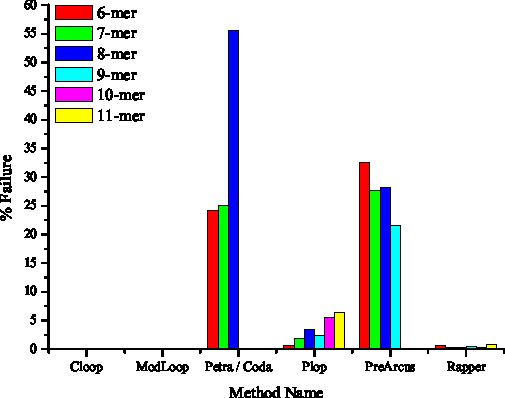
\includegraphics[width=0.85\textwidth]{08-MethodComparison/meth_fail/meth_fail.pdf}
  \end{center}
  \caption{Per loop-length, the percentage of loops for which a given method failed to produce valid structural output.}
\label{fig:methcomp:fail_rate}
\end{figure}


\begin{figure}[hptb]
  \begin{center}
  
    \mbox{  
    
            \subfigure[\cloop]{\vspace{0.5cm}\scalebox{0.47}{
            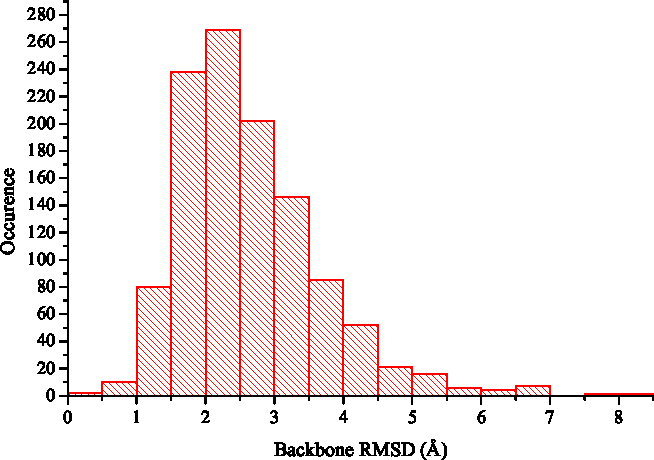
\includegraphics[width=0.884\textwidth]{08-MethodComparison/compare_bb/bb_6_Cloop.pdf}
            }}
            
            \quad
  
            \subfigure[\prearcus]{\scalebox{0.47}{
            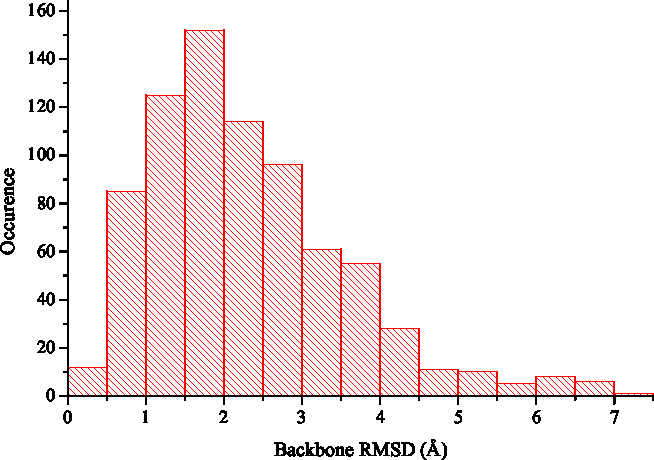
\includegraphics[width=0.884\textwidth]{08-MethodComparison/compare_bb/bb_6_PreArcus.pdf}
            }}
            
    } \mbox{ 
            
            \subfigure[\petra]{\scalebox{0.47}{
            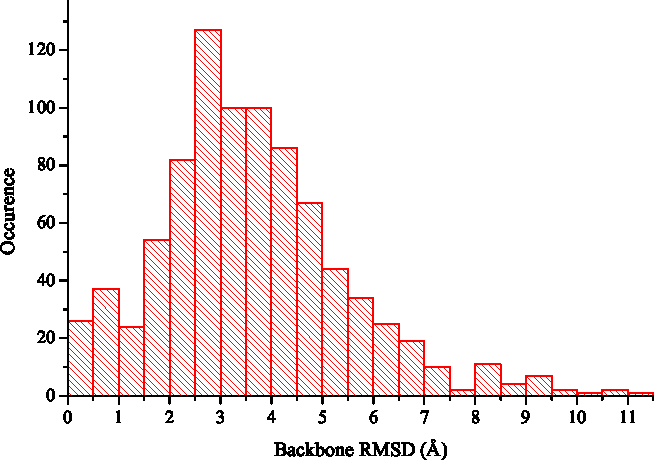
\includegraphics[width=0.884\textwidth]{08-MethodComparison/compare_bb/bb_6_Petra.pdf}
            }}
    
            \quad
    
            \subfigure[\coda]{\scalebox{0.47}{
            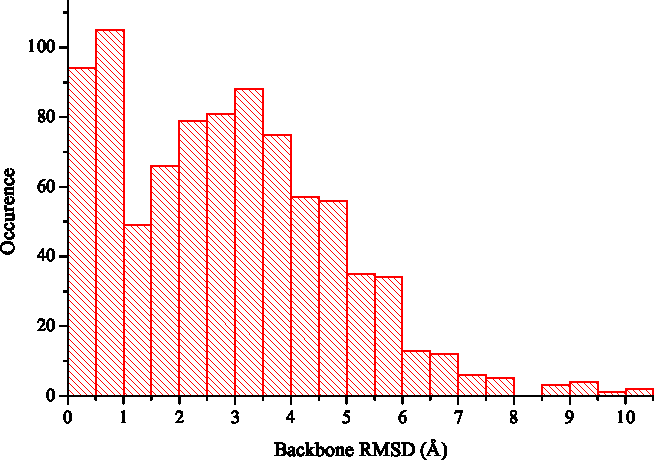
\includegraphics[width=0.884\textwidth]{08-MethodComparison/compare_bb/bb_6_Coda.pdf}
            }}
            
    } 
    \mbox{
        
            \subfigure[\rapper]{\scalebox{0.47}{
            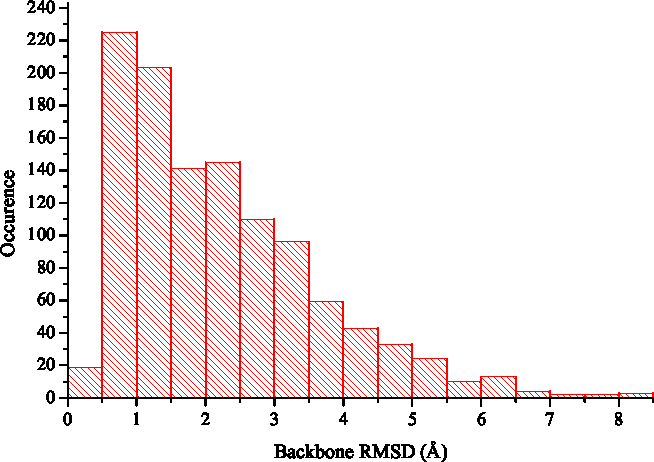
\includegraphics[width=0.884\textwidth]{08-MethodComparison/compare_bb/bb_6_Rapper.pdf}
            }} 
    
            \quad
    
            \subfigure[\plop]{\scalebox{0.47}{
            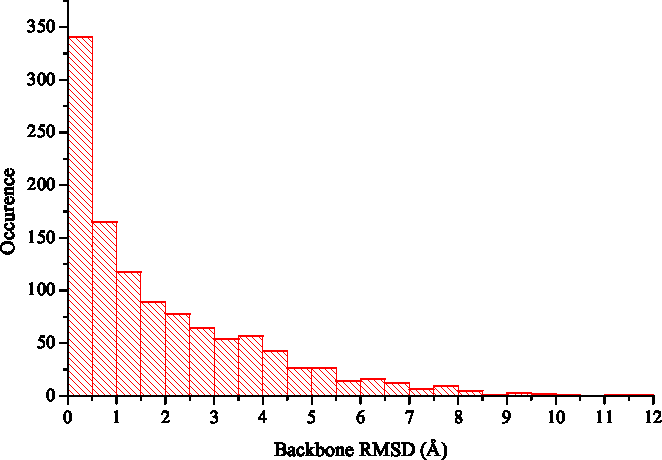
\includegraphics[width=0.884\textwidth]{08-MethodComparison/compare_bb/bb_6_plop.pdf}
            }}
    }    
    \mbox{
        
            \subfigure[\modloop\ - MolPDF]{\scalebox{0.47}{
            \includegraphics[width=0.884\textwidth]{08-MethodComparison/compare_bb/bb_6_Modeller_MolPDF.pdf}
            }} 
    
            \quad
    
            \subfigure[\modloop\ - Dope]{\scalebox{0.47}{
            \includegraphics[width=0.884\textwidth]{08-MethodComparison/compare_bb/bb_6_Modeller_Dope.pdf}
            }}
    }   

    \caption[Histogramatic distributions representing the backbone-atom \crms\ scores of the lowest 
    energy model for each \mer{6} loop prediction.]{
    Histogramatic distributions representing the \mainchain\ atom \crms\ scores of the lowest 
    energy model for each \mer{6} loop prediction. One graph is shown for each loop modelling 
    method tested during this work.}
    
    \label{fig:methcomp:hist_dist_bb_6}
    
  \end{center}
\end{figure}

\begin{figure}[hptb]
  \begin{center}
  
    \mbox{  
    
            \subfigure[\cloop]{\vspace{0.5cm}\scalebox{0.47}{
            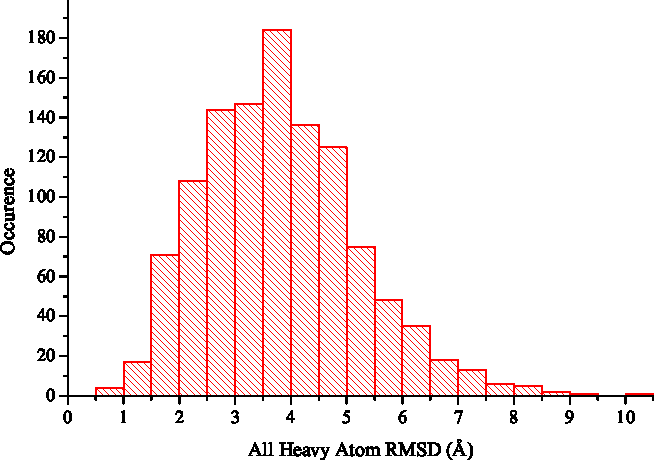
\includegraphics[width=0.884\textwidth]{08-MethodComparison/compare/aa_6_Cloop.pdf}
            }}
            
            \quad
  
            \subfigure[\prearcus]{\scalebox{0.47}{
            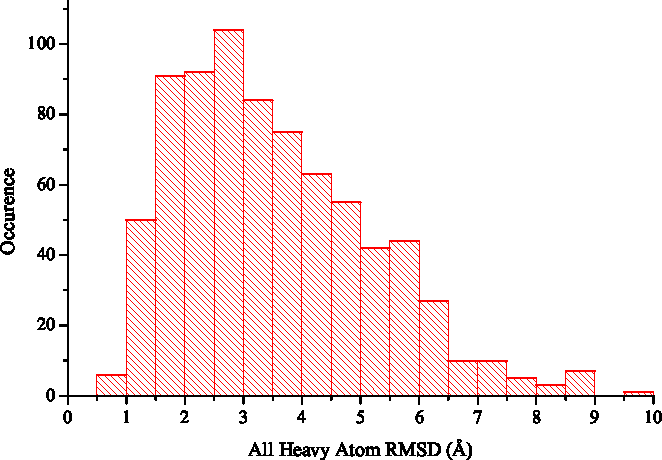
\includegraphics[width=0.884\textwidth]{08-MethodComparison/compare/aa_6_PreArcus.pdf}
            }}
            
    } \mbox{ 
            
            \subfigure[\petra]{\scalebox{0.47}{
            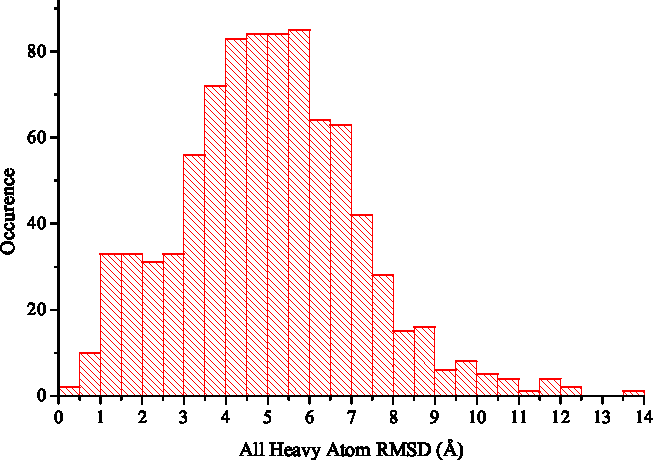
\includegraphics[width=0.884\textwidth]{08-MethodComparison/compare/aa_6_Petra.pdf}
            }}
    
            \quad
    
            \subfigure[\coda]{\scalebox{0.47}{
            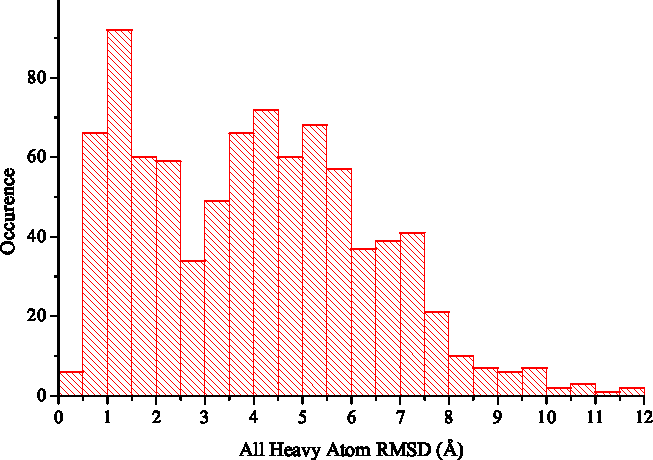
\includegraphics[width=0.884\textwidth]{08-MethodComparison/compare/aa_6_Coda.pdf}
            }}
            
    } 
    \mbox{
        
            \subfigure[\rapper]{\scalebox{0.47}{
            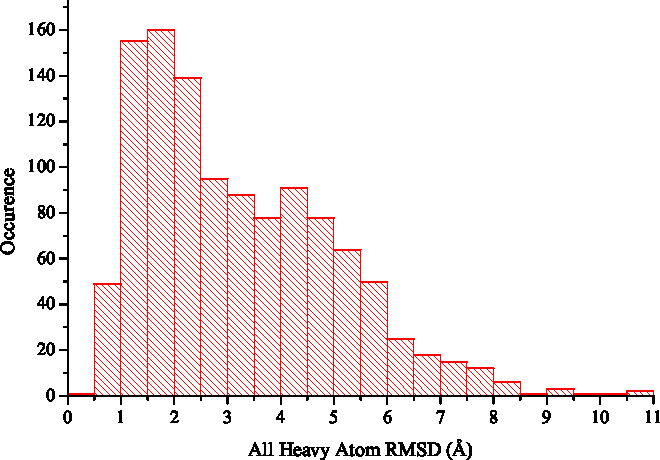
\includegraphics[width=0.884\textwidth]{08-MethodComparison/compare/aa_6_Rapper.pdf}
            }} 
    
            \quad
    
            \subfigure[\plop]{\scalebox{0.47}{
            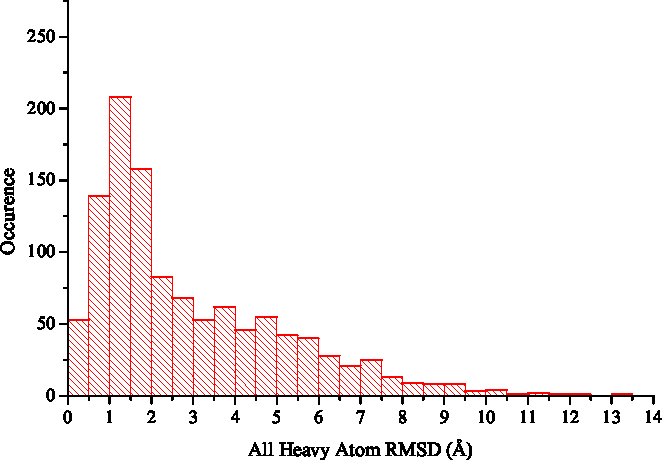
\includegraphics[width=0.884\textwidth]{08-MethodComparison/compare/aa_6_plop.pdf}
            }}
    }    
    \mbox{
        
            \subfigure[\modloop\ - MolPDF]{\scalebox{0.47}{
            \includegraphics[width=0.884\textwidth]{08-MethodComparison/compare/aa_6_Modeller_MolPDF.pdf}
            }} 
    
            \quad
    
            \subfigure[\modloop\ - Dope]{\scalebox{0.47}{
            \includegraphics[width=0.884\textwidth]{08-MethodComparison/compare/aa_6_Modeller_Dope.pdf}
            }}
    }   

    \caption[Histogramatic distributions representing the heavy-atom \crms\  scores of the lowest 
    energy model for each \mer{6} loop prediction.]{Histogramatic distributions representing the heavy-atom \crms\  scores of the lowest 
    energy model for each \mer{6} loop prediction. One graph is shown for each loop modelling 
    method tested during this work.}
    
    \label{fig:methcomp:hist_dist_ha_6}
    
  \end{center}
\end{figure}

\begin{figure}[hptb]
  \begin{center}
  
    \mbox{  
    
            \subfigure[\cloop]{\vspace{0.5cm}\scalebox{0.47}{
            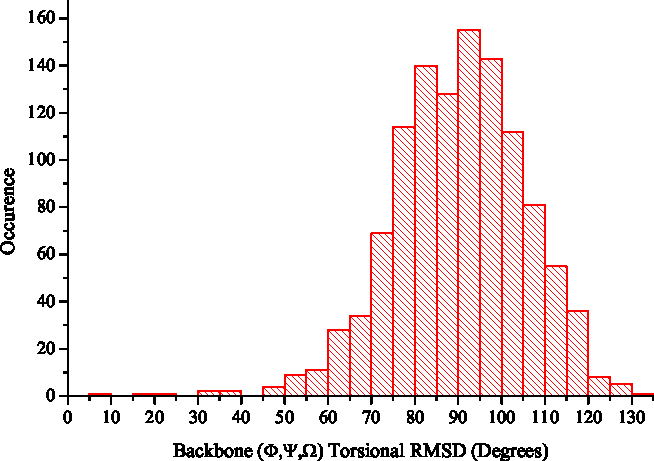
\includegraphics[width=0.884\textwidth]{08-MethodComparison/compare_bba/bba_6_Cloop.pdf}
            }}
            
            \quad
  
            \subfigure[\prearcus]{\scalebox{0.47}{
            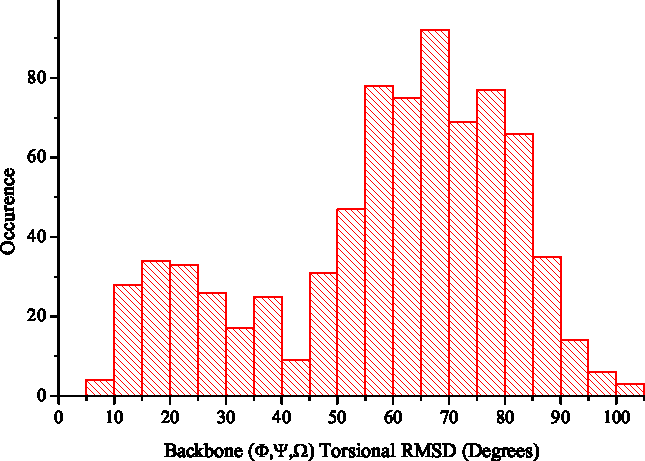
\includegraphics[width=0.884\textwidth]{08-MethodComparison/compare_bba/bba_6_PreArcus.pdf}
            }}
            
    } \mbox{ 
            
            \subfigure[\petra]{\scalebox{0.47}{
            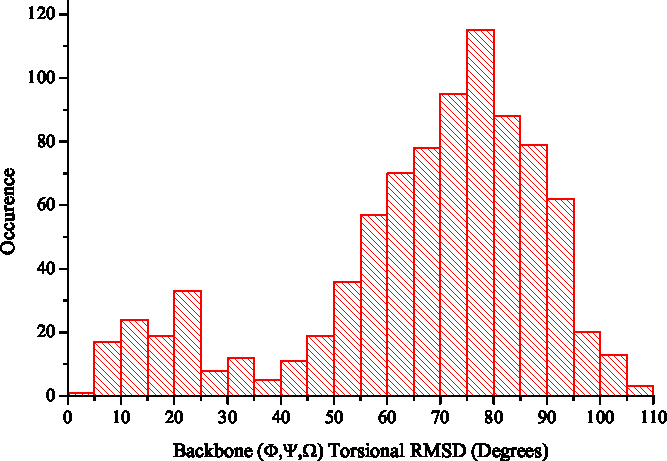
\includegraphics[width=0.884\textwidth]{08-MethodComparison/compare_bba/bba_6_Petra.pdf}
            }}
    
            \quad
    
            \subfigure[\coda]{\scalebox{0.47}{
            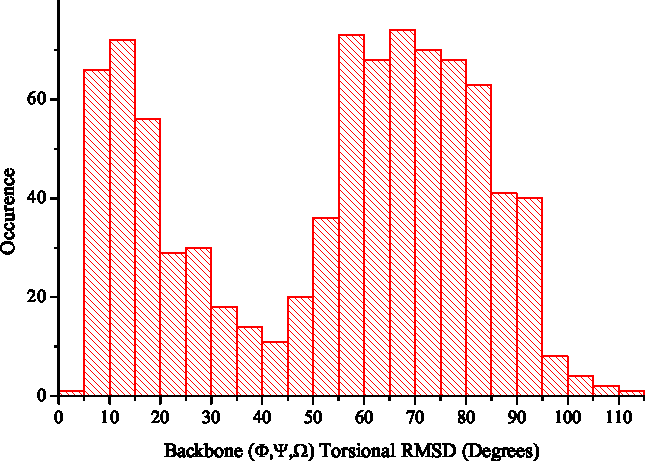
\includegraphics[width=0.884\textwidth]{08-MethodComparison/compare_bba/bba_6_Coda.pdf}
            }}
            
    } 
    \mbox{
        
            \subfigure[\rapper]{\scalebox{0.47}{
            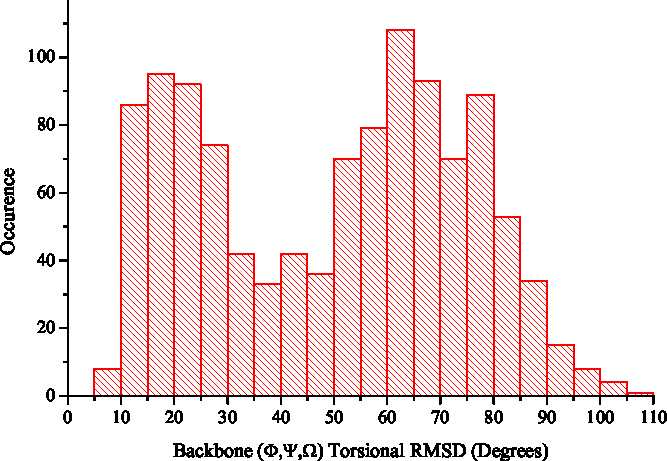
\includegraphics[width=0.884\textwidth]{08-MethodComparison/compare_bba/bba_6_Rapper.pdf}
            }} 
    
            \quad
    
            \subfigure[\plop]{\scalebox{0.47}{
            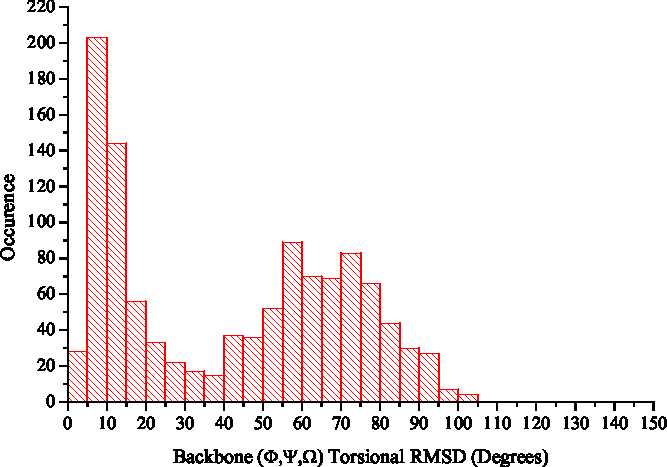
\includegraphics[width=0.884\textwidth]{08-MethodComparison/compare_bba/bba_6_plop.pdf}
            }}
    }    
    \mbox{
        
            \subfigure[\modloop\ - MolPDF]{\scalebox{0.47}{
            \includegraphics[width=0.884\textwidth]{08-MethodComparison/compare_bba/bba_6_Modeller_MolPDF.pdf}
            }} 
    
            \quad
    
            \subfigure[\modloop\ - Dope]{\scalebox{0.47}{
            \includegraphics[width=0.884\textwidth]{08-MethodComparison/compare_bba/bba_6_Modeller_Dope.pdf}
            }}
    }   

    \caption[Histogramatic distributions for the backbone torsional RMSD ($\Phi$,$\Psi$,$\Omega$) scores 
    of the lowest energy model for each \mer{6} loop prediction.]{Histogramatic distributions for the backbone torsional RMSD ($\Phi$,$\Psi$,$\Omega$) scores 
    of the lowest energy model for each \mer{6} loop prediction. One graph is shown for each loop modelling 
    method tested during this work.}
    
    \label{fig:methcomp:hist_dist_bba_6}
    
  \end{center}
\end{figure}


\begin{figure}[hptb]
  \begin{center}
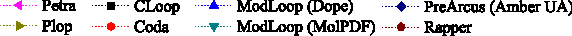
\includegraphics[width=0.7\textwidth]{08-MethodComparison/summary/key.pdf}\\[0.1cm]
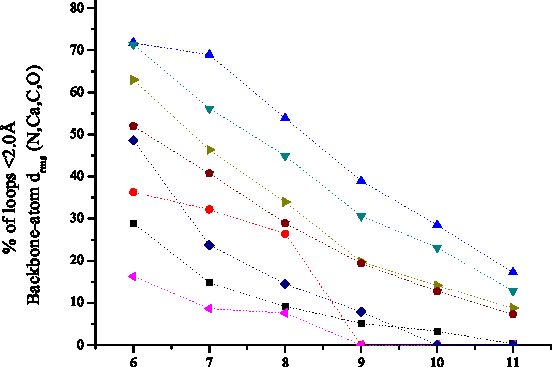
\includegraphics[width=0.7\textwidth]{08-MethodComparison/summary/backbone.pdf}
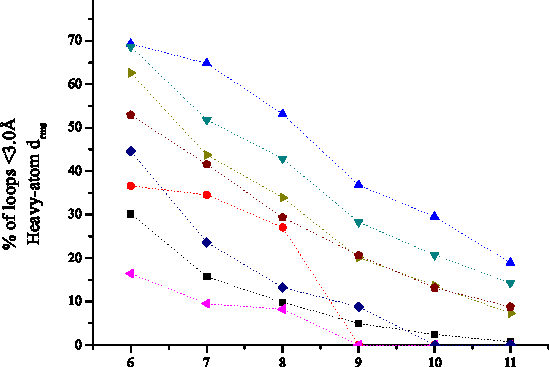
\includegraphics[width=0.7\textwidth]{08-MethodComparison/summary/heavyatom.pdf}
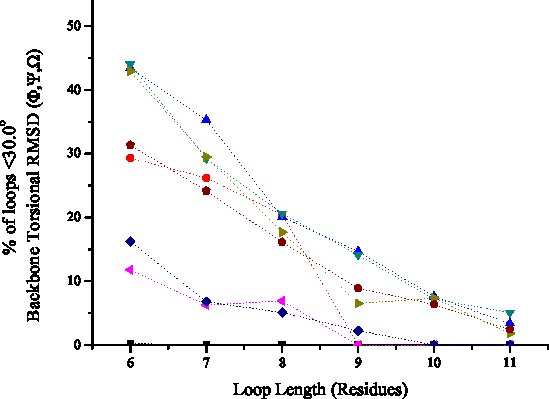
\includegraphics[width=0.7\textwidth]{08-MethodComparison/summary/torsion.pdf}
  \end{center}
  \caption{The collated analysis of prediction quality for all \abinitio\ loop modelling  methods.}
\label{fig:methcomp:summary_graph}
\end{figure}



%%%%%%%%%%%%%%%%%%%%%%%%%
\section{Data Discussion}
%%%%%%%%%%%%%%%%%%%%%%%%%

Figure \ref{fig:methcomp:summary_graph} illustrates that prediction quality, measured by the percentage of sufficiently native-like predictions, decreases approximately linearly with loop length. This decay is unsurprising as conformational space increases exponentially with each increase in loop length; as has been reported by numerous other authors. In addition, the performance-ratio between methods remains largely constant with increasing loop length -- that is to say, the relative rank of each method is predominantly the same for all loop lengths. The exception to this observation is \coda, which shows a less pronounced performance decrease with increasing loop length. It, therefore, performs comparatively better as length increases up to and including its  \mer{8} maximum.
This is most likely due to strong native-like biases originating fundamentally from its use of PDB-derived structures.






\subsection{Backbone and Heavy-atom RMSD plots}

There is essentially no relative difference between the \mainchain\ and heavy-atom \crms\ plots.
The general conclusions to draw from both are essentially the same, with one small exception.
\plop\ shows a significantly superior distribution when considering only the \mainchain\ atoms, with a large \% of structures showing \textless0.5\AA\ \crms\ to the native structure (see raw-data in appendix \ref{appendix:methcompraw}). This suggests that its main difficulty is in \emph{surface} \sidechain\ prediction, as incorrect core-facing \sidechains\ would not allow such native-like backbone placement.
Indeed, as the conformation of surface \sidechains\ can often be dramatically influenced by the crystal packing environment, these predictions can be deemed to be essentially flawless. This observation is also the only technical flaw in ranking provided by the summary graphs presented in figure \ref{fig:methcomp:summary_graph}  --   In terms of the percentage
below cutoff, \modloop\ performs significantly better, however in terms of the smaller number of flawless predictions \plop\ is clearly superior.



\subsection{Main-chain Torsional RMSD plots}

Each torsional distribution seems to be approximately bi-modal. In general there is a tight peak for native-like conformations at $\sim$15\degree\ and a wider non-native spread centring around $\sim$70\degree\ for all methods. It is worth mentioning here that \cloop\ shows essentially no native-like signal in its torsional distribution and the mode of its distribution lies at around the $\sim$90\degree\ mark. It is the view of this author that this distribution essentially represents the distribution one would obtain by the generation of completely random geometries which happen to bridge two anchor points. This also neatly proves that it is indeed possible to get very low Cartesian \crms\ structures which show very poor native-like properties in torsional space.
  

\subsection{Method Failure Rate}

Cloop is based upon the very robust \charmm\ simulation framework and a comparatively simple minimisation protocol and therefore shows no method failures. \modloop, the best performing method, also appears to be highly robust with no failures.

\rapper\ is also in general very robust showing only a small number of application errors and printing ``General Error'' in its output. There ware also some sampling errors whereby ``No models could be generated under the provided restraints'' would be printed; although obviously the only restraints imposed were the native steric interactions with the protein body and the anchor residue geometries.

\plop\ generated few errors, with the frequency seeming to increase with loop length. Most of these errors were due to the failure of the internal minimisation procedure, both generating nonsense output and log files of up to the file system limit of 2\gb\ as the error was repeatedly reported.
Some
additional rare errors also occurred with messages such as ``atom out of cell bounds''. This type of error reflects the fact that \plop\ makes increased use of rule-based tests over each of \cloop, \modloop\ and \rapper\ -- which are more susceptible to failure on unusual input.

\prearcus\ displayed failure rates of between 25\% and 33\%, almost exclusively due to sampling failures, although one isolated case was due to a minor error detected by the program during the generation of the surface atom list.
The sampling failure-rate is discussed further in section 
\ref{section:methcomp:prearcus:final_remarks}. The code itself has demonstrated itself to be robust, having undergone no application crashes.

The failure rate of \petra\ and \coda\ is the highest amongst all methods, being up to 55\% for 8 residue loops. They also exhibit the greatest variety of reasons for failure; symptomatic of the comparative complexity of the modelling procedure, in the use of eight separate applications. Segmentation faults were worryingly frequent, most often occurring in  \textsc{Fread} and \textsc{Read7}, being suggestive of poor underlying software engineering practices. The remainder of the errors were in sampling within the default cutoffs, where often no valid loop candidates could be identified.
Additional very frequent errors occurred during the processing of the applications licence with its licence server -- these however, in no way contribute to the method failure percentage as they were circumvented by \emph{repeatedly} re-running the entire modelling procedure until the licence checks passed for all eight applications in turn.


\subsection{Comparing All Distributions}

With the previous observations in mind, it can be said that in general \abinitio\ predictions are of excellent quality for loops of 6 or 7 residues in length. The best methods show a significant bias towards highly native-like states in both Cartesian and torsional space. Although \coda,\ the token PDB-derived method, performs well in terms of percentage; one has to take its poor failure rate into account. It can clearly be seen that when \coda\ chooses a fragment, there is native-like bias, however a failure rate of \textgreater50\% is impractical for real-world modelling usage. It is also highly likely that increasing the cutoffs used by the application to allow less likely candidates would merely reduce the quality of prediction to a useless level. As such it is clear that \abinitio\ methods are genuinely of superior use in the prediction of medium-length loop structures.


For 8 and 9 residue loops, although Cartesian \crms\ values remain low, the percentage of models with native-like torsions shows a significant decrease for all methods. This is most likely due the exponential increase in geometric possibilities -- defined by conformations that will bridge the available gap using populated Ramachandran regions, without clashing with the protein body.
As such, structural filters are of less use and it is the final score of the forcefield that is required to provide increasing discrimination. It is certainly interesting that above 7 residues in length, the \textsc{Dope} \emph{statistical} potential used by \modloop\ is of real value in selecting the most native-like predictions.

Sadly, even for the top-performing methods, the conformational search of loops of both 10 and 11 residues in length on average proves too difficult, with only a 6\% prediction rate for the best method on \mer{11} structures.
Clearly for these structures, the scope of the conformational search has to grow by orders of magnitude, in order to capture native-like states with any consistent accuracy.


%%%%%%%%%%%%%%%%%%%%%%%%%%%%%%%%%%%%
\section{ Conclusions and Comments for each Method}
%%%%%%%%%%%%%%%%%%%%%%%%%%%%%%%%%%%%


From this critical method comparison, it is clear that within the chosen set of methods some methods perform significantly better than others. The overall ranking is shown in table \ref{table:methcomp:methodrank}. There are a number of traits that seem to generally either lead to success or failure.
In the following section, each method is considered individually and comments made where appropriate. Following this, more general conclusions are drawn and the traits of an idealised loop modelling application are discussed in section \ref{section:methcomp:final_remarks}.

\begin{table}[htbp]
\begin{center}
\begin{tabular}{l+c}
\toprule
Rank & Name \\
\midrule
\first  & \modloop  \\
\second & \plop     \\
\third  & \rapper   \\
\xth{4} & \coda$^*$ \\
\xth{5} & \prearcus \\
\xth{6} & \petra    \\
\xth{7} & \cloop    \\
\bottomrule
\end{tabular}
\end{center}
\caption[The overall method ranking]{The overall method ranking, as judged by the scoring criteria used in this comparison. $^*$Note that \coda\ is not an \abinitio\ method, as it uses PDB-derived structural fragments. It is presented here only as a reference state for comparison with \abinitio\ methods.}
\label{table:methcomp:methodrank}
\end{table}


%%%%%%%%%%%%%%%%%%%
\subsection{CLoop}
%%%%%%%%%%%%%%%%%%%

The original \cloop\ calibration was far from comprehensive. 1,000 candidate models were generated for each of only 32 loop conformations -- 10 loops for lengths 4, 8 and 12 residues from Fisers' test set\cite{METHOD:Fis2000} and two additional long loops of length 17 and 30 residues. \cloop\ shows relatively poor performance in this study compared to the author values. By contrast to other studies, the authors quote either minimum or average RMSD visited from the 1,000 model ensemble as their main performance benchmarks, as opposed to the RMSD of the single minimum energy structure. The authors also quote the RMSD for the whole protein and not just the loop atoms, again resulting in their lower values. It was noted in the original work that no near-native structures were sampled for their pair of long loops.

The authors note that a particular strength of \cloop\ is its ability to rapidly generate all-atom models as opposed to backbone-only models in a similar time to that of other backbone-only methods. \cloop, however, shows an especially poor native-like Ramachandran bias in its final models. This is likely due to its na\"ive use of highly randomised \phipsi\ pairings; obliterating any bias towards native-like structures that its coarse-grained parametised \phipsi\ pairings provide. \cloop\ also relies \emph{heavily} on the properties of its minimisation protocol both to close loop branches whose termini exhibit high separation in Cartesian space and also to resolve massive steric clashes both within the loop itself and with the protein surface.


%%%%%%%%%%%%%%%%%%%%%
\subsection{ModLoop}
%%%%%%%%%%%%%%%%%%%%%

\modloop\ has been shown to consistently be the best current loop modelling method, outperforming all others for all loop lengths. Interestingly, the supplied \textsc{Dope} statistical potential performs almost identically for \mer{6} loops structures when compared to \textsc{MolPDF}, but gives a significant increase in selection accuracy for all other tested loop lengths.


%%%%%%%%%%%%%%%%%%%%%%%%
\subsection{Orchestrar}
%%%%%%%%%%%%%%%%%%%%%%%%

\subsubsection{Coda}

As all test-cases used in this study are derived from the PDB, the fragments corresponding to the majority of loops should be present within the \textsc{Fread} database and therefore should be available for selection. This obviously isn't a fair test of its ability in a real comparative modelling application. It is presented for completeness and as a measure of the methods ability to select a loop if a perfect example should be present in its database. It is noteworthy that the \sidechain\ coordinates of the fragments are not present in the database, therefore, the prediction of \sidechain\ orientation still has to be correctly performed even if the correct main-chain fragment is selected.
Baring this in mind, it is unsurprising that \coda\ shows better overall performance than \petra. What is much more interesting is that \coda\ is significantly outperformed by three \abinitio\ methods.

\subsubsection{Petra}

As the published method \textsc{Petra} is actually used as part of the \orchestrar\ suite of applications, it is not trivial to automate loop modelling. For this work two 100 line scripts were produced calling a total of 8 separate \textsc{Orchestrar} applications to generate each \abinitio\ loop model; there is no built-in automated way provided. This makes computation difficult and susceptible to errors as if any of the eight applications fails to run to completion, the automated run must be re-executed. In addition to this a multitude of superfluous output files are created in the process which must be managed between successive \textsc{Orchestrar} applications in any automated script. 

A second factor which makes \textsc{Petra} less suited to cluster computation is the large 3\gb\ APD which, to avoid heavy network traffic, must be replicated locally across the computer cluster and subsequently maintained and synchronised with any updates.

Finally and most importantly, \textsc{Petra} has three fundamental limitations. Firstly, there is no sequence dependence within the APD as the \phipsi\ pairs are the same for every residue type. Secondly, the database ignores the \Omg\ backbone
torsion and therefore cannot encode  cis-residues. Thirdly, although the database encodes \mer{12} fragments, due to the requirement for two anchor residues for  stitching the loop onto the protein core, only loops of up to 8 residues in length can be modelled.
\petra\ is, therefore, fundamentally not able to model a significant subset of loop conformations.



%%%%%%%%%%%%%%%%%%
\subsection{PLOP}
\label{section:methcomp:plopConclude}
%%%%%%%%%%%%%%%%%%

It is clear that \plop\ is highly capable in producing high-quality native-like predictions, reflecting the abilities of this hierarchical protocol described in the original publication. There are, however, a number of differences between the performance analysis reported here for \plop\ and that quoted in the original publication\cite{METHOD:Plop}. Such differences are listed here for completeness.

It is of note that the original published performance analysis used information on the crystal packing environment from the PDB file. The asymmetric unit was recreated for each loop by including atoms from the other copies of the protein within 20\AA. The models were identical for each copy of the chain and energy calculations were preformed in the knowledge of all chains. The authors note that this crystal packing is important for selecting viable loop conformations. It is worth noting, however, that no knowledge of the nature of the asymmetric unit is present when creating a comparative model and therefore such information was not used in the comparison from this work. It is also noteworthy that there are many cases of proteins of both identical and highly homologous sequences, that are crystallised with fundamentally different asymmetric units, dependent upon the exact crystallisation conditions.

Secondly, it is noted in the original paper\cite{METHOD:Plop} that an additional step of refinement beyond the standard protocol was used in their benchmark. For each loop they performed the whole loop build protocol multiple times. To reduce the sensitivity of the results to the chosen steric parameters, the procedure was repeated for steric overlap ratios of 0.7 and 0.75. The five best conformations from both of these runs were then used as starting conformations for further runs with \ca\ positions restrained to within 4\AA\ of their initial conformation. These results were then recombined with the initial runs and re-run a final time with 2.0\AA\ distance restraints. This was not used in this work, as such a process is not a documented built-in functionality of \plop\ and would require significant scripts to be written. It was noted that this only had an effect on loops of 8 residues or more in length.

Finally, the data-set used for the \plop\ analysis was filtered to remove all those states that interacted with a ligand, contained disproportionate amounts of secondary structure or had any moderately severe steric clash.
This is not the case for this comparison, where such loops are still present within the test-set.







%%%%%%%%%%%%%%%%%%%%%%
\subsection{Pre-Arcus}
\label{section:methcomp:prearcus:final_remarks}
%%%%%%%%%%%%%%%%%%%%%%



As described in chapter \ref{chapter:reduced_rep}, \prearcus\ exhaustively and rapidly enumerates all possible conformers for each loop test-structure; subsequently filtering conformations which either clash with the protein body or for which the end-joining distance is too great. To perform this filtering, empirical cutoffs were employed to ensure that, on average, at least one native-torsional-bin conformer is kept without retaining too many other candidates. This practise was used to ensure that the stage 2 and 3 refinement steps were computationally tractable. Unfortunately, however, fixed cut-offs result in too great a variation in the number of retained conformers for each loop test-case; for some loops tens of structures were selected, for others tens of thousands were retained. In hindsight, this observation is expected with the highly variable degree of conformational flexibility found in native loop structures. 

Compared to other methods, \prearcus\ also shows a comparatively high failure rate; unsuccessful in finding any valid conformation for  between one quarter and one third of loop test-cases. The low numbers of conformers under cut-off for some loop-test cases  goes towards an explanation for why this failure rate is comparatively high. A second major disadvantage of the exhaustive enumeration is its high cost for loop lengths above nine residues. At this loop length, so many conformers are kept which are under filter cut-offs, that whilst the method is still feasible for single loops on a standard desktop computer, the calibration against the entire database was not computationally viable. To combat these imbalances, the search method needs to become adaptive, tuning the conformer selection process by the current loop flexibility. 

 


It is true that \prearcus, whilst demonstrating good Cartesian \crms\ scores for many shorter loops, shows comparatively poor torsional properties. This is interesting as  the \prearcus\ conformational search is focused around torsional manipulation. It is likely that \prearcus\ utilises the shape of the protein surface to effectively guide loop conformation selection, giving low Cartesian \crms\ as the correct overall path is followed. As \prearcus\ uses a coarse-grained backbone representation, it is evident that too many native-like conformations are filtered early in the conformational generation procedure.
It is concluded that this is due to the ``lever-effect'', meaning that relatively small torsional deviations at the beginning of a loop structure can result in large Cartesian deviations at the loop terminus. This, in turn, means that the closest conformers in torsional space may well exhibit strong atomic clashes or large loop-closure distances. If there is no valid native-torsional-bin conformer, which does occur, conformations will be accepted which are non-native-like in torsional space, but which are within the allowable Cartesian space. 

 It is thought that \prearcus, perhaps, relies too heavily on its torsional minimisation protocol to resolve steric conflict. It is true that stage 1 of the loop modelling process can generate structures which have mild contact with the protein body. It may also generate structures which do not have sufficient space to include the required \sidechains, as no checks are performed for this situation. Upon torsional minimisation, the driving force of these undesirable contacts is to propel the loop away from the body of the protein. This is a compelling reason for the disproportionate generation of overly-extended loop conformations by \prearcus.
In light of this, as stage 2 is comparatively far more computationally expensive than stage 1, it is likely that an increase in the complexity of the \angleset\ and a concurrent decrease in filter cutoffs will actually increase efficiency, as fewer unsuccessful minimisations will be performed.

Finally, even if overly-extended structures are generated, it would be hoped that the chosen \forcefield\ would screen against such conformations. Unfortunately, \amberwgbsa\ as discussed in section \ref{section:casp:salt_bridge_discussion}, appears to discriminate poorly against these conformations; especially when favourable electrostatic interactions have been formed. As previously concluded, \forcefield\ adjustments are evidently required in order to shift the balance against electrostatically-driven interactions.


%%%%%%%%%%%%%%%%%%%%%%
\subsection{Rapper}
%%%%%%%%%%%%%%%%%%%%%%

All generated
conformers followed three fundamental rules to guarantee
local structural competency: near-ideal geometry, residue-specific
\phipsi\ propensities and excluded volume. These
rules can be regarded as negative filters that specify which
conformers are forbidden.
By the authors own admission, the final energy evaluator -- \textsc{Rapdf} -- is evidently inferior to third generation molecular mechanics forcefields like \ambergbsa\ in selection of final models. This is the most likely explanation for the moderate reduction in performance of \rapper\ over that of both \plop\ and \modloop.



%%%%%%%%%%%%%%%%%%%%%%%%
\section{Final Remarks}
\label{section:methcomp:final_remarks}
%%%%%%%%%%%%%%%%%%%%%%%%

Within this study, \modloop\ emerges as the leader for loop modelling, closely followed by \plop. Both outperform other methods by all chosen criteria, however, \plop\ is surpassed by \modloop\ in Cartesian space. Interestingly, both methods are based on entirely different underlying algorithms and operate approximately within the same total computational execution time.
Also, each one can be deemed ``more \abinitio''\ by different criteria. \plop\ used an \abinitio\ scoring function (\opls\  and \gbsa), but then generates conformations using a filter-centric decision-based selection process with a complex clustering algorithm.
\modloop\ on the other hand uses knowledge-based statistical potentials with few physical qualities, but uses predominantly newtonian MD and simulated annealing as its optimisation method.

It is certainly interesting that both \petra\ and \prearcus\ show very similar success in torsional space; perhaps unsurprising, as they are both based on very similar underlying coarse-grained torsional libraries. What is also interesting is that \prearcus\ seems significantly better than \petra\ at following native-like paths in Cartesian space. This is probably due to its use of its torsional minimisation protocol which would allow the loops to be guided over the protein surface.
It is important to note that whilst \petra\ is limited to \mer{8} loops by the size of its database, the design choice of an on-the-fly building procedure for \prearcus\ completely\ removes this limitation.
In light of this \prearcus\ can be deemed the most successful coarse \angleset\ method in this critical comparison.

\subsection{The Granularity of the Main-chain Torsional Search}
 
It is clear that more fine-grained backbone angle libraries ultimately lead to superior predictions -- \rapper\ and \plop\ both utilise fine-grained libraries and \modloop\ uses statistical potentials based on a fine-grained Ramachandran grid. By contrast, both \prearcus\ and \petra\ show similar performance in torsional space; both being based on similar underlying backbone representations and both of which show comparatively poorer performance.
A larger fine-grained backbone torsion library, of course, requires an efficient sampling procedure. However, such a  library also gives a better chance that more native-like conformations can be found.  What is certainly true, is that a large fraction of larger backbone libraries can potentially be pre-screened on-the-fly early in the conformational search by very computationally cheap and efficient procedures -- such as simple steric tests.
The
cost of larger libraries is, therefore, smaller than it may first seem.

An important trait of most modelling applications is that almost all neglect the cis-proline conformation.
On one hand this is surprising as this work has already described that 6\% of proline residues are in a cis conformation in native protein structure and of these up to 13\% of loops contain a cis-proline.  On the other hand inclusion of this additional torsion complicates both the search procedure and the internal method implementation and parametisation.

\subsection{Structural Filtering}

Rule-based filters have an important role to play in increasing efficiency, by ensuring that no nonsense structures
are sent for evaluation by more detailed and therefore computationally expensive calculations.
Such filters should remain largely simple and based on either geometry, physical effects or statistical weights. It is essential that such filters do not remove any native-like candidates during the pre-refinement stages of the modelling process.

\subsection{ Consensus Approaches}

Consensus methods such as \coda, whilst sometimes leading to improvements in prediction quality, do not tackle the underlying limitations of prediction accuracy; namely the coverage of conformational space or the representation of the energy landscape. In general, it is the view of this author that such methods are an attempt to polish otherwise failing  methodologies.
Time is most likely better spent on the enhancement of the underlying physical model and conformational sampling efficiency, as opposed to perfecting a vast quantity of rule-based filters.
This view is shared by others, especially in light of the temporary closure of some web-based prediction servers during the \casp-7 competition, to prevent their use by competing consensus-servers.

\subsection{The Crystal Environment}

It has been noted\cite{METHOD:Plop} that crystal structures often contain moderate steric clashes. This can be ascribed to incomplete model refinement, although others would argue with that conclusion. What is certainly true is that loop modelling methods should screen such structures out at an early stage for efficiency. Therefore, candidate models generated for native loops with steric clashes will most likely exhibit disproportionately high RMSD values when compared to the native state. Although minimisation will have removed these clashes, alternative conformations may now be more energetically favourable than a compacted native-like loop model.

Crystal packing forces were partially discussed earlier in relation to \plop\ in section \ref{section:methcomp:plopConclude}. Such forces have previously been shown to play a significant role in the conformation of loops and of the \sidechains\ connected to them\cite{METHOD:Plop:Jacobson2002A}. These are not normally simulated in loop modelling methods. This would require either some sort of periodic boundary, or multiple copies of the protein loop and core to be included. Defining too many additional atoms is unfeasible in terms of computational cost. In any case, during real comparative modelling, information about the unit cell is not available. In the future, more ``extreme''  comparative modelling may well require the simulation of multiple potential crystallographic lattices, in order to ensure the accuracy of surface predictions. 


\subsection{Protonation States}

\Sidechain\ protonation states are an important determinant for the balance between competing energetic minima in loop structure prediction. This is due to factors such as electrostatic interactions between charged \sidechains. There are proven cases where \sidechains, especially histidine residues, can exist in multiple ionisation states at the same pH, dependent upon their local environment. It is also true that \xray\ structures are not crystalised solely at biologically relevant pHs. Accurate assignment of ionisation state to titratable groups is a body of work in itself. Incorrectly assigned ionisation states contribute to very significant energetic errors and therefore incorrect model structures.
Thus, protonation states
require attention for any future work. This will most likely involve dynamic changes during the course of the simulation. 








